\documentclass[]{tufte-book}

% ams
\usepackage{amssymb,amsmath}

\usepackage{ifxetex,ifluatex}
\usepackage{fixltx2e} % provides \textsubscript
\ifnum 0\ifxetex 1\fi\ifluatex 1\fi=0 % if pdftex
  \usepackage[T1]{fontenc}
  \usepackage[utf8]{inputenc}
\else % if luatex or xelatex
  \makeatletter
  \@ifpackageloaded{fontspec}{}{\usepackage{fontspec}}
  \makeatother
  \defaultfontfeatures{Ligatures=TeX,Scale=MatchLowercase}
  \makeatletter
  \@ifpackageloaded{soul}{
     \renewcommand\allcapsspacing[1]{{\addfontfeature{LetterSpace=15}#1}}
     \renewcommand\smallcapsspacing[1]{{\addfontfeature{LetterSpace=10}#1}}
   }{}
  \makeatother

\fi

% graphix
\usepackage{graphicx}
\setkeys{Gin}{width=\linewidth,totalheight=\textheight,keepaspectratio}

% booktabs
\usepackage{booktabs}

% url
\usepackage{url}

% hyperref
\usepackage{hyperref}

% units.
\usepackage{units}


\setcounter{secnumdepth}{-1}

% citations
\usepackage{natbib}
\bibliographystyle{plainnat}


% pandoc syntax highlighting
\usepackage{color}
\usepackage{fancyvrb}
\newcommand{\VerbBar}{|}
\newcommand{\VERB}{\Verb[commandchars=\\\{\}]}
\DefineVerbatimEnvironment{Highlighting}{Verbatim}{commandchars=\\\{\}}
% Add ',fontsize=\small' for more characters per line
\newenvironment{Shaded}{}{}
\newcommand{\AlertTok}[1]{\textcolor[rgb]{1.00,0.00,0.00}{\textbf{#1}}}
\newcommand{\AnnotationTok}[1]{\textcolor[rgb]{0.38,0.63,0.69}{\textbf{\textit{#1}}}}
\newcommand{\AttributeTok}[1]{\textcolor[rgb]{0.49,0.56,0.16}{#1}}
\newcommand{\BaseNTok}[1]{\textcolor[rgb]{0.25,0.63,0.44}{#1}}
\newcommand{\BuiltInTok}[1]{#1}
\newcommand{\CharTok}[1]{\textcolor[rgb]{0.25,0.44,0.63}{#1}}
\newcommand{\CommentTok}[1]{\textcolor[rgb]{0.38,0.63,0.69}{\textit{#1}}}
\newcommand{\CommentVarTok}[1]{\textcolor[rgb]{0.38,0.63,0.69}{\textbf{\textit{#1}}}}
\newcommand{\ConstantTok}[1]{\textcolor[rgb]{0.53,0.00,0.00}{#1}}
\newcommand{\ControlFlowTok}[1]{\textcolor[rgb]{0.00,0.44,0.13}{\textbf{#1}}}
\newcommand{\DataTypeTok}[1]{\textcolor[rgb]{0.56,0.13,0.00}{#1}}
\newcommand{\DecValTok}[1]{\textcolor[rgb]{0.25,0.63,0.44}{#1}}
\newcommand{\DocumentationTok}[1]{\textcolor[rgb]{0.73,0.13,0.13}{\textit{#1}}}
\newcommand{\ErrorTok}[1]{\textcolor[rgb]{1.00,0.00,0.00}{\textbf{#1}}}
\newcommand{\ExtensionTok}[1]{#1}
\newcommand{\FloatTok}[1]{\textcolor[rgb]{0.25,0.63,0.44}{#1}}
\newcommand{\FunctionTok}[1]{\textcolor[rgb]{0.02,0.16,0.49}{#1}}
\newcommand{\ImportTok}[1]{#1}
\newcommand{\InformationTok}[1]{\textcolor[rgb]{0.38,0.63,0.69}{\textbf{\textit{#1}}}}
\newcommand{\KeywordTok}[1]{\textcolor[rgb]{0.00,0.44,0.13}{\textbf{#1}}}
\newcommand{\NormalTok}[1]{#1}
\newcommand{\OperatorTok}[1]{\textcolor[rgb]{0.40,0.40,0.40}{#1}}
\newcommand{\OtherTok}[1]{\textcolor[rgb]{0.00,0.44,0.13}{#1}}
\newcommand{\PreprocessorTok}[1]{\textcolor[rgb]{0.74,0.48,0.00}{#1}}
\newcommand{\RegionMarkerTok}[1]{#1}
\newcommand{\SpecialCharTok}[1]{\textcolor[rgb]{0.25,0.44,0.63}{#1}}
\newcommand{\SpecialStringTok}[1]{\textcolor[rgb]{0.73,0.40,0.53}{#1}}
\newcommand{\StringTok}[1]{\textcolor[rgb]{0.25,0.44,0.63}{#1}}
\newcommand{\VariableTok}[1]{\textcolor[rgb]{0.10,0.09,0.49}{#1}}
\newcommand{\VerbatimStringTok}[1]{\textcolor[rgb]{0.25,0.44,0.63}{#1}}
\newcommand{\WarningTok}[1]{\textcolor[rgb]{0.38,0.63,0.69}{\textbf{\textit{#1}}}}

% table with pandoc

% multiplecol
\usepackage{multicol}

% strikeout
\usepackage[normalem]{ulem}

% morefloats
\usepackage{morefloats}


% tightlist macro required by pandoc >= 1.14
\providecommand{\tightlist}{%
  \setlength{\itemsep}{0pt}\setlength{\parskip}{0pt}}

% title / author / date
\title{Modelaje Epidemiológico en \texttt{R}}
\author{Rodrigo Zepeda}
\date{2022-08-14}


\begin{document}

\maketitle




\hypertarget{r}{%
\chapter{\texorpdfstring{¿\texttt{R}?}{¿R?}}\label{r}}

Yo me enfrenté a \texttt{R} por primera vez hace más de 8 años cuando un
grupo de investigadores con quienes trabajaba compartieron su código en
\texttt{R}. Fue horrible. El código estaba mal comentado, elaborado sin
ninguna lógica de programación (yo, según esto, ya sabía programar en
ese entonces) y no funcionaba. Quizá, si ya conoces el programa, tu
experiencia ha sido similar: en general cuando nos enfrentamos a
\texttt{R} nos enfrentamos a cosas que otras personas escribieron para
salir del aprieto sin mucha explicación. ¡Es lo peor del mundo porque no
se entiende nada! El propósito de estas notas (¿y clase?) es dual:
acompañarte en un acercamiento a \texttt{R} desde cero y perderle el
miedo a dicho programa.

\begin{marginfigure}

\includegraphics[width=150px]{images/rlogo} \caption[`R` es un programa chido de estadística]{`R` es un programa chido de estadística. FIN.}\label{fig:unnamed-chunk-1}
\end{marginfigure}

Una de las primeras cosas que necesitamos saber es que \texttt{R} (por
más que sus más ávidos defensores digan lo contrario) no es para todo.
Si tú ya conoces otro lenguaje (sea \texttt{Stata}, \texttt{Excel},
\texttt{SAS}, etc) sabrás utilizar muchas de sus opciones. Estoy seguro
que, de conocer uno de estos, te será muchísimo más fácil seguir sacando
promedios en tu lenguaje favorito que en \texttt{R}, realizar
regresiones lineales es probablemente más sencillo en \texttt{Stata}
mientras que las gráficas de barras quizá te sean más simples en
\texttt{Excel}. Lo que probablemente no sea más sencillo de hacer en
otro lenguaje (salvo si tu otro lenguaje es \texttt{Python},
\texttt{Julia} ó \texttt{Matlab}) es realizar modelos de simulación
desde cero y todo el análisis que conlleva. Para eso, \texttt{R} es,
indiscutiblemente, una de las mejores opciones para quienes no conocen
de programación\footnote{Modelos de simulación más avanzados suelen
  hacerse en \texttt{C}, \texttt{C++} o \texttt{Fortran} por su
  velocidad; empero, es necesario conocer más de programación.}.

Finalmente, uno de los consejos más importantes que te puedo dar es que
este curso no te va a servir si no practicas. Igual que como pasa con
los idiomas uno no aprende \texttt{R} en una semana \emph{sin
practicarlo después}. Mi sugerencia es que, a la vez que sigues estas
notas comiences a trabajar un proyecto \emph{tuyo} específico junto con
\href{https://duckduckgo.com/}{el buscador de Internet de tu
preferencia} a la mano y empieces a usar \texttt{R} en él.
Practica\footnote{La práctica hace al maestro}.

\hypertarget{algunas-ventajas-de-r-y-cosas-no-tan-padres}{%
\section{\texorpdfstring{Algunas ventajas de \texttt{R} y cosas no tan
padres}{Algunas ventajas de R y cosas no tan padres}}\label{algunas-ventajas-de-r-y-cosas-no-tan-padres}}

\hypertarget{puntos-a-favor-de-r}{%
\subsection{\texorpdfstring{Puntos a favor de
\texttt{R}}{Puntos a favor de R}}\label{puntos-a-favor-de-r}}

\begin{itemize}
\item
  Todo el mundo lo usa (7o lenguaje más usado según
  \href{https://pypl.github.io/PYPL.html}{PyPl} y 16
  \href{https://www.tiobe.com/tiobe-index/}{según TIOBE}). Quizá éste es
  el punto más a favor. Si mucha gente lo conoce y lo utiliza, hay más
  opciones de ayuda. Los sitios de StackOverflow
  \href{https://stackoverflow.com}{en inglés} y
  \href{https://es.stackoverflow.com}{en español} son excelentes para
  pedir apoyo en \texttt{R}; los
  \href{https://groups.google.com/forum/\#!forum/r-help-archive}{grupos
  de usuarios de Google} son otra fuente muy buena así como
  \href{https://r-contributors.slack.com}{el canal de Slack}. Entre más
  gente usa el programa; es más fácil obtener ayuda porque seguro
  alguien más tuvo hace ya tiempo el mismo problema que tú.
\item
  Hay grupos interesantes que valen la pena mencionar:
  \href{https://rladies.org/}{Rladies} que busca promoveer la diversidad
  de género entre quienes usan \texttt{R},
  \href{https://rainbowr.netlify.app/}{RainbowR} con el objetivo de
  promover y conectar a la banda LGBTQ+ que trabaja en \texttt{R}.
\item
  Todas las personas que trabajan en estadística publican sus métodos y
  su código en \texttt{R} (eso, claro, cuando publican sus métodos). Es
  raro encontrar \emph{un nuevo método estadístico} en el mundo y que no
  se pueda usar, de alguna forma, en \texttt{R}.
\item
  Dentro de los lenguajes de programación \texttt{R} es de los más
  sencillos. Quienes lo hicieron realmente se preocuparon por su público
  (de no especialistas) y en general desarrollan para él.
\item
  \texttt{R} es gratis. Y en esta época de austeridad, cualquier ahorro
  es bueno.
\item
  Todo lo que se hace en \texttt{R} es público. \texttt{R} no tiene
  métodos secretos ni es una caja negra. Todo lo que hace cada una de
  las funciones de \texttt{R}, cualquiera lo puede revisar, por
  completo.
\item
  En \texttt{R} puedes hacer notas ¡como estas! donde guardes todo tu
  trabajo, reportes automatizados e incluso
  \href{https://gallery.shinyapps.io/086-bus-dashboard/}{documentos
  interactivos} para facilitar el análisis de datos.
\item
  \texttt{R} puede hacer gráficas bonitas:
\end{itemize}

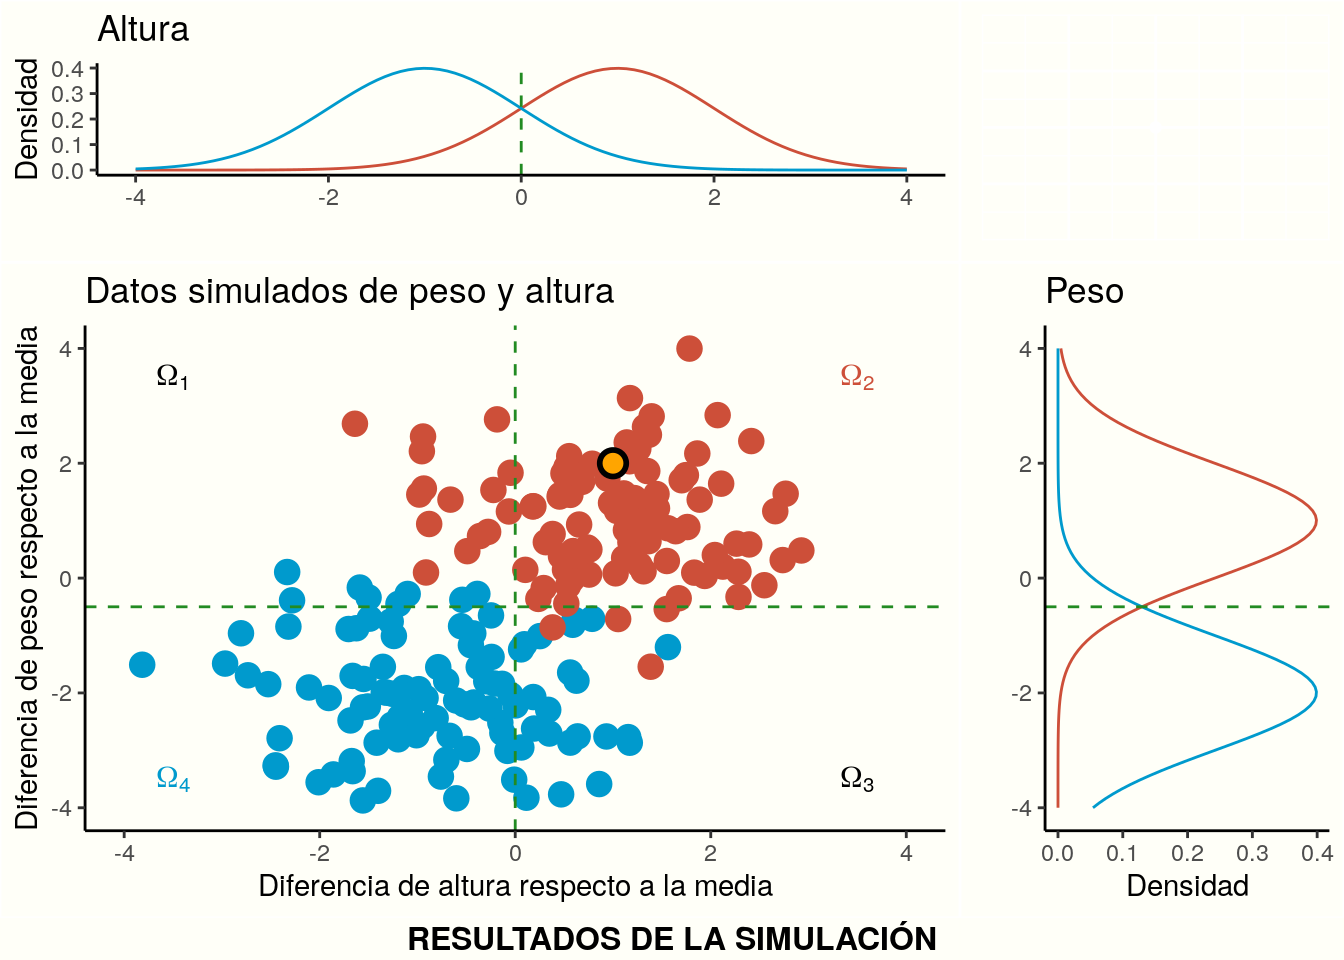
\includegraphics{Introducción_a_R_files/figure-latex/unnamed-chunk-2-1}

Por supuesto, no todo es miel sobre hojuelas con \texttt{R}.
Particularmente, algunos de los problemas con el lenguaje:

\begin{marginfigure}
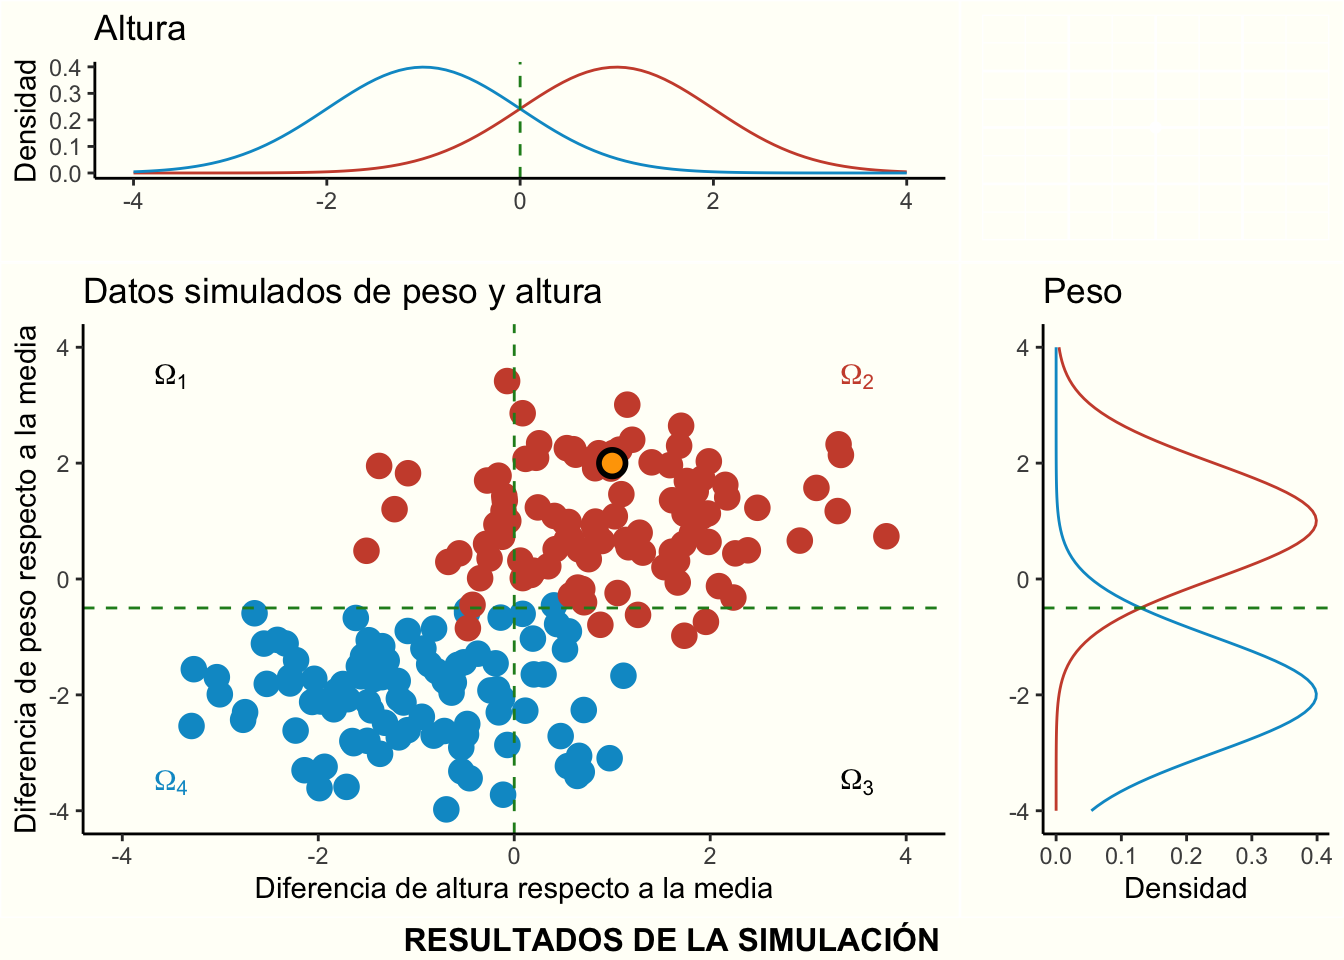
\includegraphics{Introducción_a_R_files/figure-latex/unnamed-chunk-3-1} \caption[La curva de aprendizaje de `R` es más empinada pero después de un rato vale la pena]{La curva de aprendizaje de `R` es más empinada pero después de un rato vale la pena}\label{fig:unnamed-chunk-3}
\end{marginfigure}

\begin{itemize}
\item
  La curva de aprendizaje es mucho más empinada que para otros programas
  estadísticos (como \texttt{Stata}, \texttt{SAS} o \texttt{SPSS})
  ¡particularmente si es tu primera vez programando!
\item
  La mayor parte de las personas que trabajan en \texttt{R} no son
  programadores de verdad. Gran parte del código que te puedes encontrar
  \textbf{en el mundo real} está escrito
  \href{https://nsaunders.wordpress.com/2014/05/14/this-is-why-code-written-by-scientists-gets-ugly/}{con
  prisa para salir del aprieto} sin mucha planeación, con pocos
  comentarios, falta de control de versiones y pocas herramientas de
  revisión. ¡Internet está lleno de
  \href{https://codegolf.stackexchange.com/a/4011}{creaturas espantosas
  escritas en \texttt{R}}!
\end{itemize}

\begin{marginfigure}
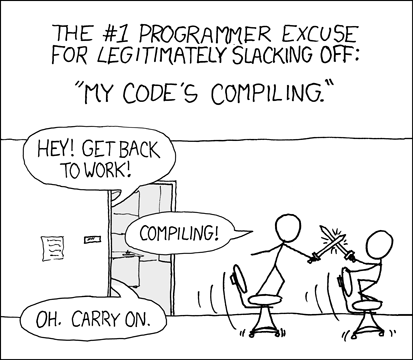
\includegraphics[width=5.74in]{images/compiling} \caption[`R` puede ser muy lento pero eso te da oportunidad de hacer otras cosas ;) ]{`R` puede ser muy lento pero eso te da oportunidad de hacer otras cosas ;) .}\label{fig:unnamed-chunk-4}
\end{marginfigure}

\begin{itemize}
\item
  \texttt{R}
  \href{https://github.com/matthieugomez/benchmark-stata-r}{de ninguna
  manera es veloz} por lo que algunos programas (lo veremos en
  simulación) pueden ser extremada (y dolorosamente) lentos.
\item
  \texttt{R} espera que tú sepas \emph{a priori} el método estadístico
  que vas a seguir. ¡A veces uno no se acuerda!
\end{itemize}

\hypertarget{bienvenidx-a-r-vigorous-calisthenics-suxed-asuxed-se-llama-esta-versiuxf3n}{%
\chapter{\texorpdfstring{Bienvenidx a \texttt{R}, Vigorous Calisthenics
(sí, así se llama esta
versión)}{Bienvenidx a R, Vigorous Calisthenics (sí, así se llama esta versión)}}\label{bienvenidx-a-r-vigorous-calisthenics-suxed-asuxed-se-llama-esta-versiuxf3n}}

\texttt{R} es un lenguaje de cómputo y un programa estadístico
\href{https://www.gnu.org/philosophy/free-sw.html}{libre}, gratuito,
\href{http://adv-r.had.co.nz/Functional-programming.html}{de
programación funcional} (¿qué es eso?),
\href{https://en.wikipedia.org/wiki/Object-oriented_programming}{orientado
a objetos} (\emph{what??}) que mutó a partir de otros dos lenguajes
conocidos como \texttt{Scheme} y \texttt{S}\footnote{De ahí que se llame
  \texttt{R} porque la \texttt{R} es una mejor letra que la \texttt{S}
  (todos lo sabemos) -Atte. Rodrigo, el autor de este documento.}. El
primero de estos fue desarrollado en el MIT por Sussman y Steele
mientras que el segundo surgió en los laboratorios Bell\footnote{Mejor
  conocidos ahora como AT\&T, la compañía celular que nunca tiene señal}
creado por Becker, Wilks y Chambers. \texttt{R}
\href{https://cran.r-project.org/doc/html/interface98-paper/paper_2.html}{nació
en junio de 1995} a partir del trabajo de Ross Ihaka y Robert
Gentleman\footnote{Sus nombres empiezan con la letra \texttt{R}
  ¿coincidencia?}.

Desde su creación, la mayor parte del desarrollo de \texttt{R} ha sido
trabajo completamente voluntario de la
\href{https://www.r-project.org/foundation/}{Fundación R}, del equipo de
R Core y de miles de usuarios que han creado funciones específicas para
\texttt{R} conocidas como paquetes (\texttt{packages}). Actualmente el
repositorio más importante de \texttt{R}, CRAN, contiene 18401 paquetes
con distintas funciones para hacer ¡lo que quieras!

Como todo el trabajo en \texttt{R} es voluntario hace falta:

\begin{enumerate}
\def\labelenumi{\arabic{enumi}.}
\item
  Una homologación en los métodos. Puedes encontrar varias funciones
  \emph{que supuestamente hacen exactamente lo mismo} (como es el caso
  de \texttt{emojifont}, \texttt{fontemoji} y \texttt{emoGG} para
  graficar usando emojis).
\item
  Estandarizar la notación. Algunos paquetes como aquellos del
  \texttt{tidyverse} (veremos más adeltna) utilizan \texttt{pipes}
  (\texttt{\%\textgreater{}\%}); estos sólo funcionan en el
  \texttt{tidyverse} pero no fuera del mismo.
\end{enumerate}

Sin embargo, también es una gran ventaja que sean los usuarios de
\texttt{R} quienes guían su desarrollo. El lenguaje va mutando según
peticiones de las personas que lo usan. Si hay algo que te gustaría
\texttt{R} tuviera y aún no existe ¡lo puedes proponer!

\hypertarget{nuestro-entorno-de-trabajo}{%
\section{Nuestro entorno de trabajo}\label{nuestro-entorno-de-trabajo}}

\hypertarget{r-1}{%
\subsection{\texorpdfstring{\texttt{R}}{R}}\label{r-1}}

\begin{marginfigure}
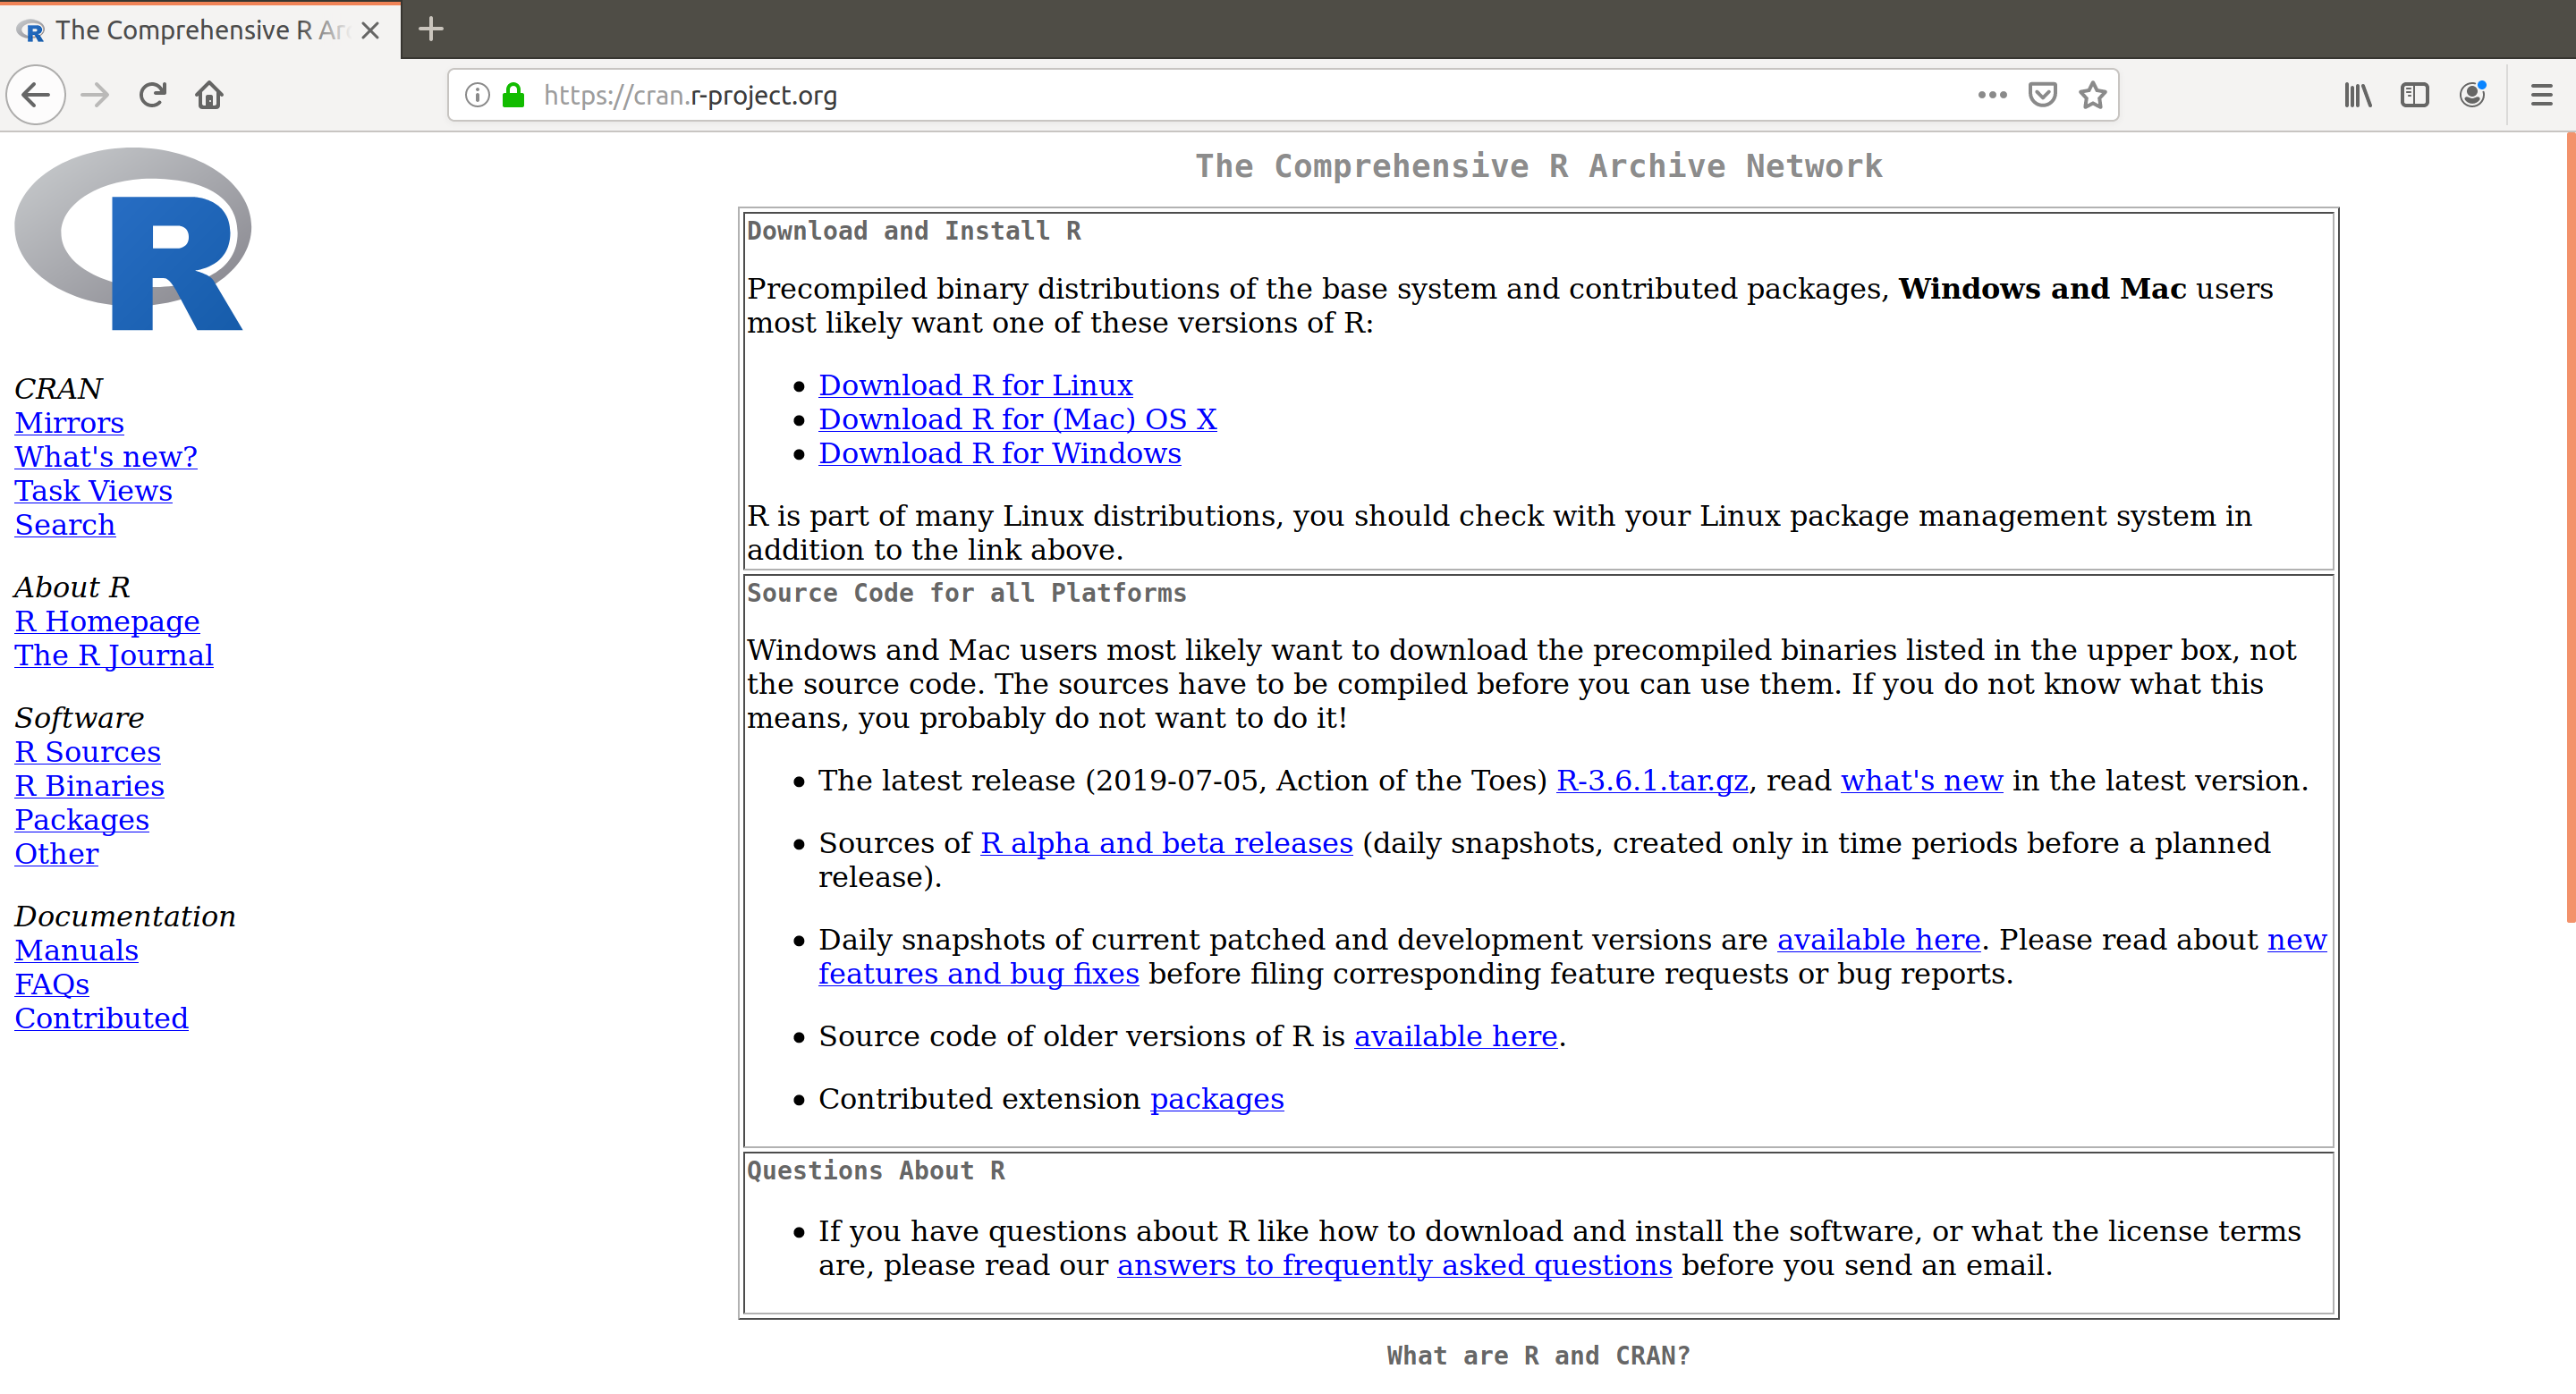
\includegraphics[width=40in]{images/CRAN1} \caption[Oficialmente, la página de `R` es de las páginas más feas del mundo]{Oficialmente, la página de `R` es de las páginas más feas del mundo. ¡No te dejes llevar por las apariencias!}\label{fig:unnamed-chunk-5}
\end{marginfigure}

A lo largo de estas notas estaré trabajando con: R version 4.2.0
(2022-04-22) \emph{Vigorous Calisthenics}. La más reciente versión de
\texttt{R} la puedes encontrar en
\href{https://cran.r-project.org}{CRAN}. Para ello ve al sitio y
selecciona tu plataforma.

\begin{marginfigure}
\textbf{Nota usuarios de Mac} En algunas Mac, al abir R, aparece el
siguiente mensaje de advertencia:

\texttt{During\ startup\ -\ Warning\ messages:\ 1:\ Setting\ LC\_CTYPE\ failed\ {[}...{]}}

para
\href{https://stackoverflow.com/questions/9689104/installing-r-on-mac-warning-messages-setting-lc-ctype-failed-using-c}{solucionarlo}
ve a \texttt{Aplicaciones} y abre \texttt{Terminal}. Copia y pega en
ella el siguiente texto:

\texttt{defaults\ write\ org.R-project.R\ force.LANG\ en\_US.UTF-8}

Da enter, cierra la \texttt{Terminal} y reinicia \texttt{R}.
\end{marginfigure}

\begin{itemize}
\item
  En el caso de Windows da clic en \texttt{Download\ R\ for\ Windows} y
  luego en \texttt{install\ R\ for\ the\ first\ time}. Finalmente,
  ejecuta el instalable que aparece al dar click en
  \texttt{Download\ R\ 4.2.0\ for\ Windows} .
\item
  En el caso de Mac selecciona \texttt{Download\ R\ for\ (Mac)\ OS\ X} y
  luego elige \texttt{R-4.2.0.pkg}. En Mac puede que necesites instalar
  adicionalmente \href{https://www.xquartz.org}{XQuartz} (según tu
  versión de Mac). Si tu Mac es una versión suficientemente antigua,
  sigue las instrucciones específicas de \texttt{CRAN}.
\end{itemize}

\begin{marginfigure}
Si tienes problemas para instalar puedes usar
\href{https://rstudio.cloud}{RStudio Cloud}.
\end{marginfigure}

\begin{itemize}
\tightlist
\item
  En el caso de Linux al elegir \texttt{Download\ R\ for\ Linux} tendrás
  la opción de buscar tu distribución específica. Al elegirla,
  aparecerán instrucciones para tu terminal de comandos; síguelas. En el
  caso de Linux, según los paquetes de \texttt{R} que elijamos instalar
  en la computadora requerirás instalar paquetería adicional para tu
  distribución de Linux. \texttt{R} te informará de la paquetería
  necesaria conforme la requiera.
\end{itemize}

\hypertarget{rstudio}{%
\subsection{RStudio}\label{rstudio}}

\begin{marginfigure}

\includegraphics[width=49.08in]{images/rstudio} \caption[RStudio es una empresa que se dedica a hacer cosas para R]{RStudio es una empresa que se dedica a hacer cosas para R.}\label{fig:unnamed-chunk-8}
\end{marginfigure}

\texttt{RStudio} es una interfaz gráfica (IDE) para \texttt{R}. Puedes
pensar a \texttt{R} como el \emph{Bloc de Notas} y a \texttt{RStudio}
como \emph{Word}. El \emph{Bloc} tiene todas las capacidades que
necesitas para poder escribir; empero, es muchísimo mejor trabajar tus
\emph{papers} en \emph{Word}. De la misma manera, \texttt{R} tiene todas
las capacidades para hacer estadística \emph{pero un formato horrible} y
\texttt{RStudio} se ha convertido en la más popular forma de usar
\texttt{R}. Por supuesto que no es la única; algunas alternativas son
\href{https://atom.io/packages/ide-r}{Atom con ide-r},
\href{https://marketplace.eclipse.org/content/statet-r}{Eclipse con
StatET} y \href{https://rkward.kde.org}{RKWard}. En general es posible
seguir estas notas sin que tengas \texttt{RStudio} pero, si es tu
primera vez programando, no lo recomiendo.

\begin{marginfigure}
Si ya tienes experiencia con lenguajes como Python, Javascript, Java ó
alguno de los mil C que existen, no tendrás ningún problema usando el
editor de tu preferencia.
\end{marginfigure}

Para descargar \texttt{RStudio} ve a \href{https://www.rstudio.com}{su
página} y da clic en \texttt{Download\ RStudio}. Baja tu pantalla hasta
donde dice \texttt{Installers\ for\ Supported\ Platforms} y elige tu
plataforma: \texttt{Windows}, \texttt{Mac\ OS\ X} ó tu sabor de
\texttt{Linux} preferido. Una vez descargado el archivo, ábrelo y sigue
las instrucciones que aparecen en pantalla.

\hypertarget{primeros-pasos-en-rstudio}{%
\chapter{\texorpdfstring{Primeros pasos en
\texttt{RStudio}}{Primeros pasos en RStudio}}\label{primeros-pasos-en-rstudio}}

Una vez hayas instalado \texttt{R} y \texttt{RStudio}, abre
\texttt{RStudio}\footnote{Si decidiste no instalar RStudio salta al
  final de esta sección.}. Te enfrentarás a una pantalla similar a esta:

\begin{figure}
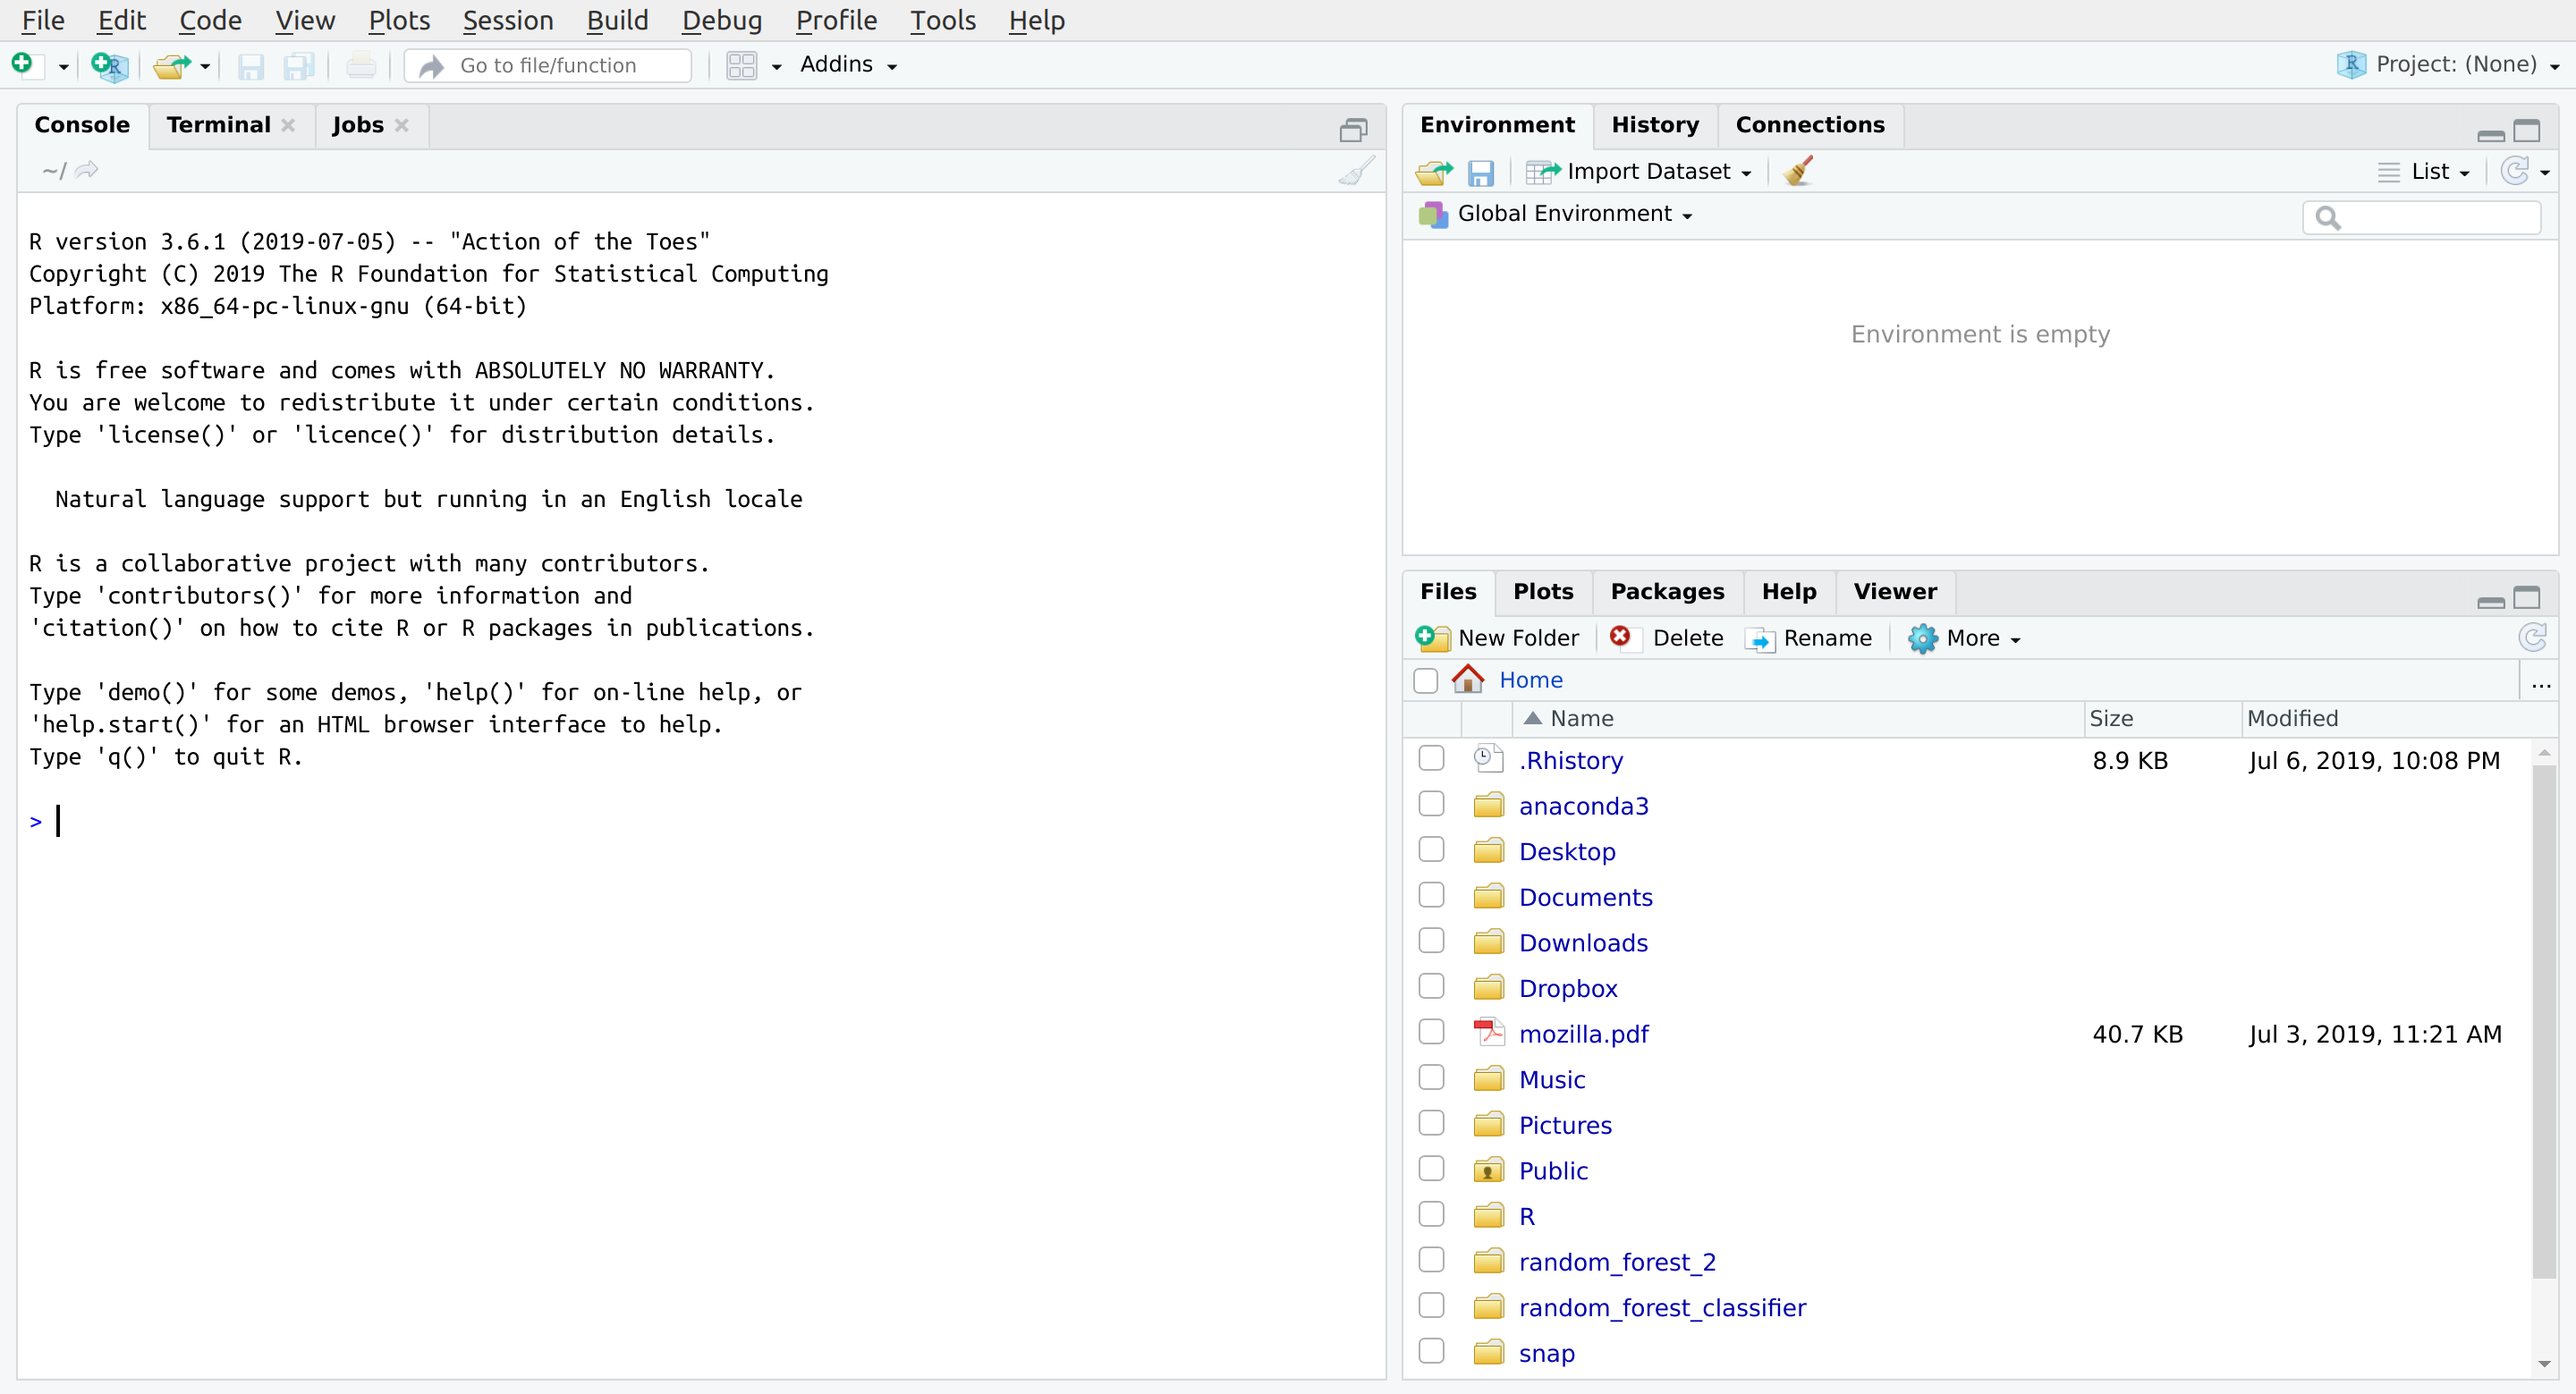
\includegraphics[width=40in]{images/RStudio1} \caption[La primera vez que abres RStudio]{La primera vez que abres RStudio}\label{fig:fig-main}
\end{figure}

Si tu RStudio tiene sólo 3 páneles, como en mi caso, ve a la esquina
superior izquierda (signo de hoja+) y elige un nuevo \texttt{R\ Script}

\begin{figure}
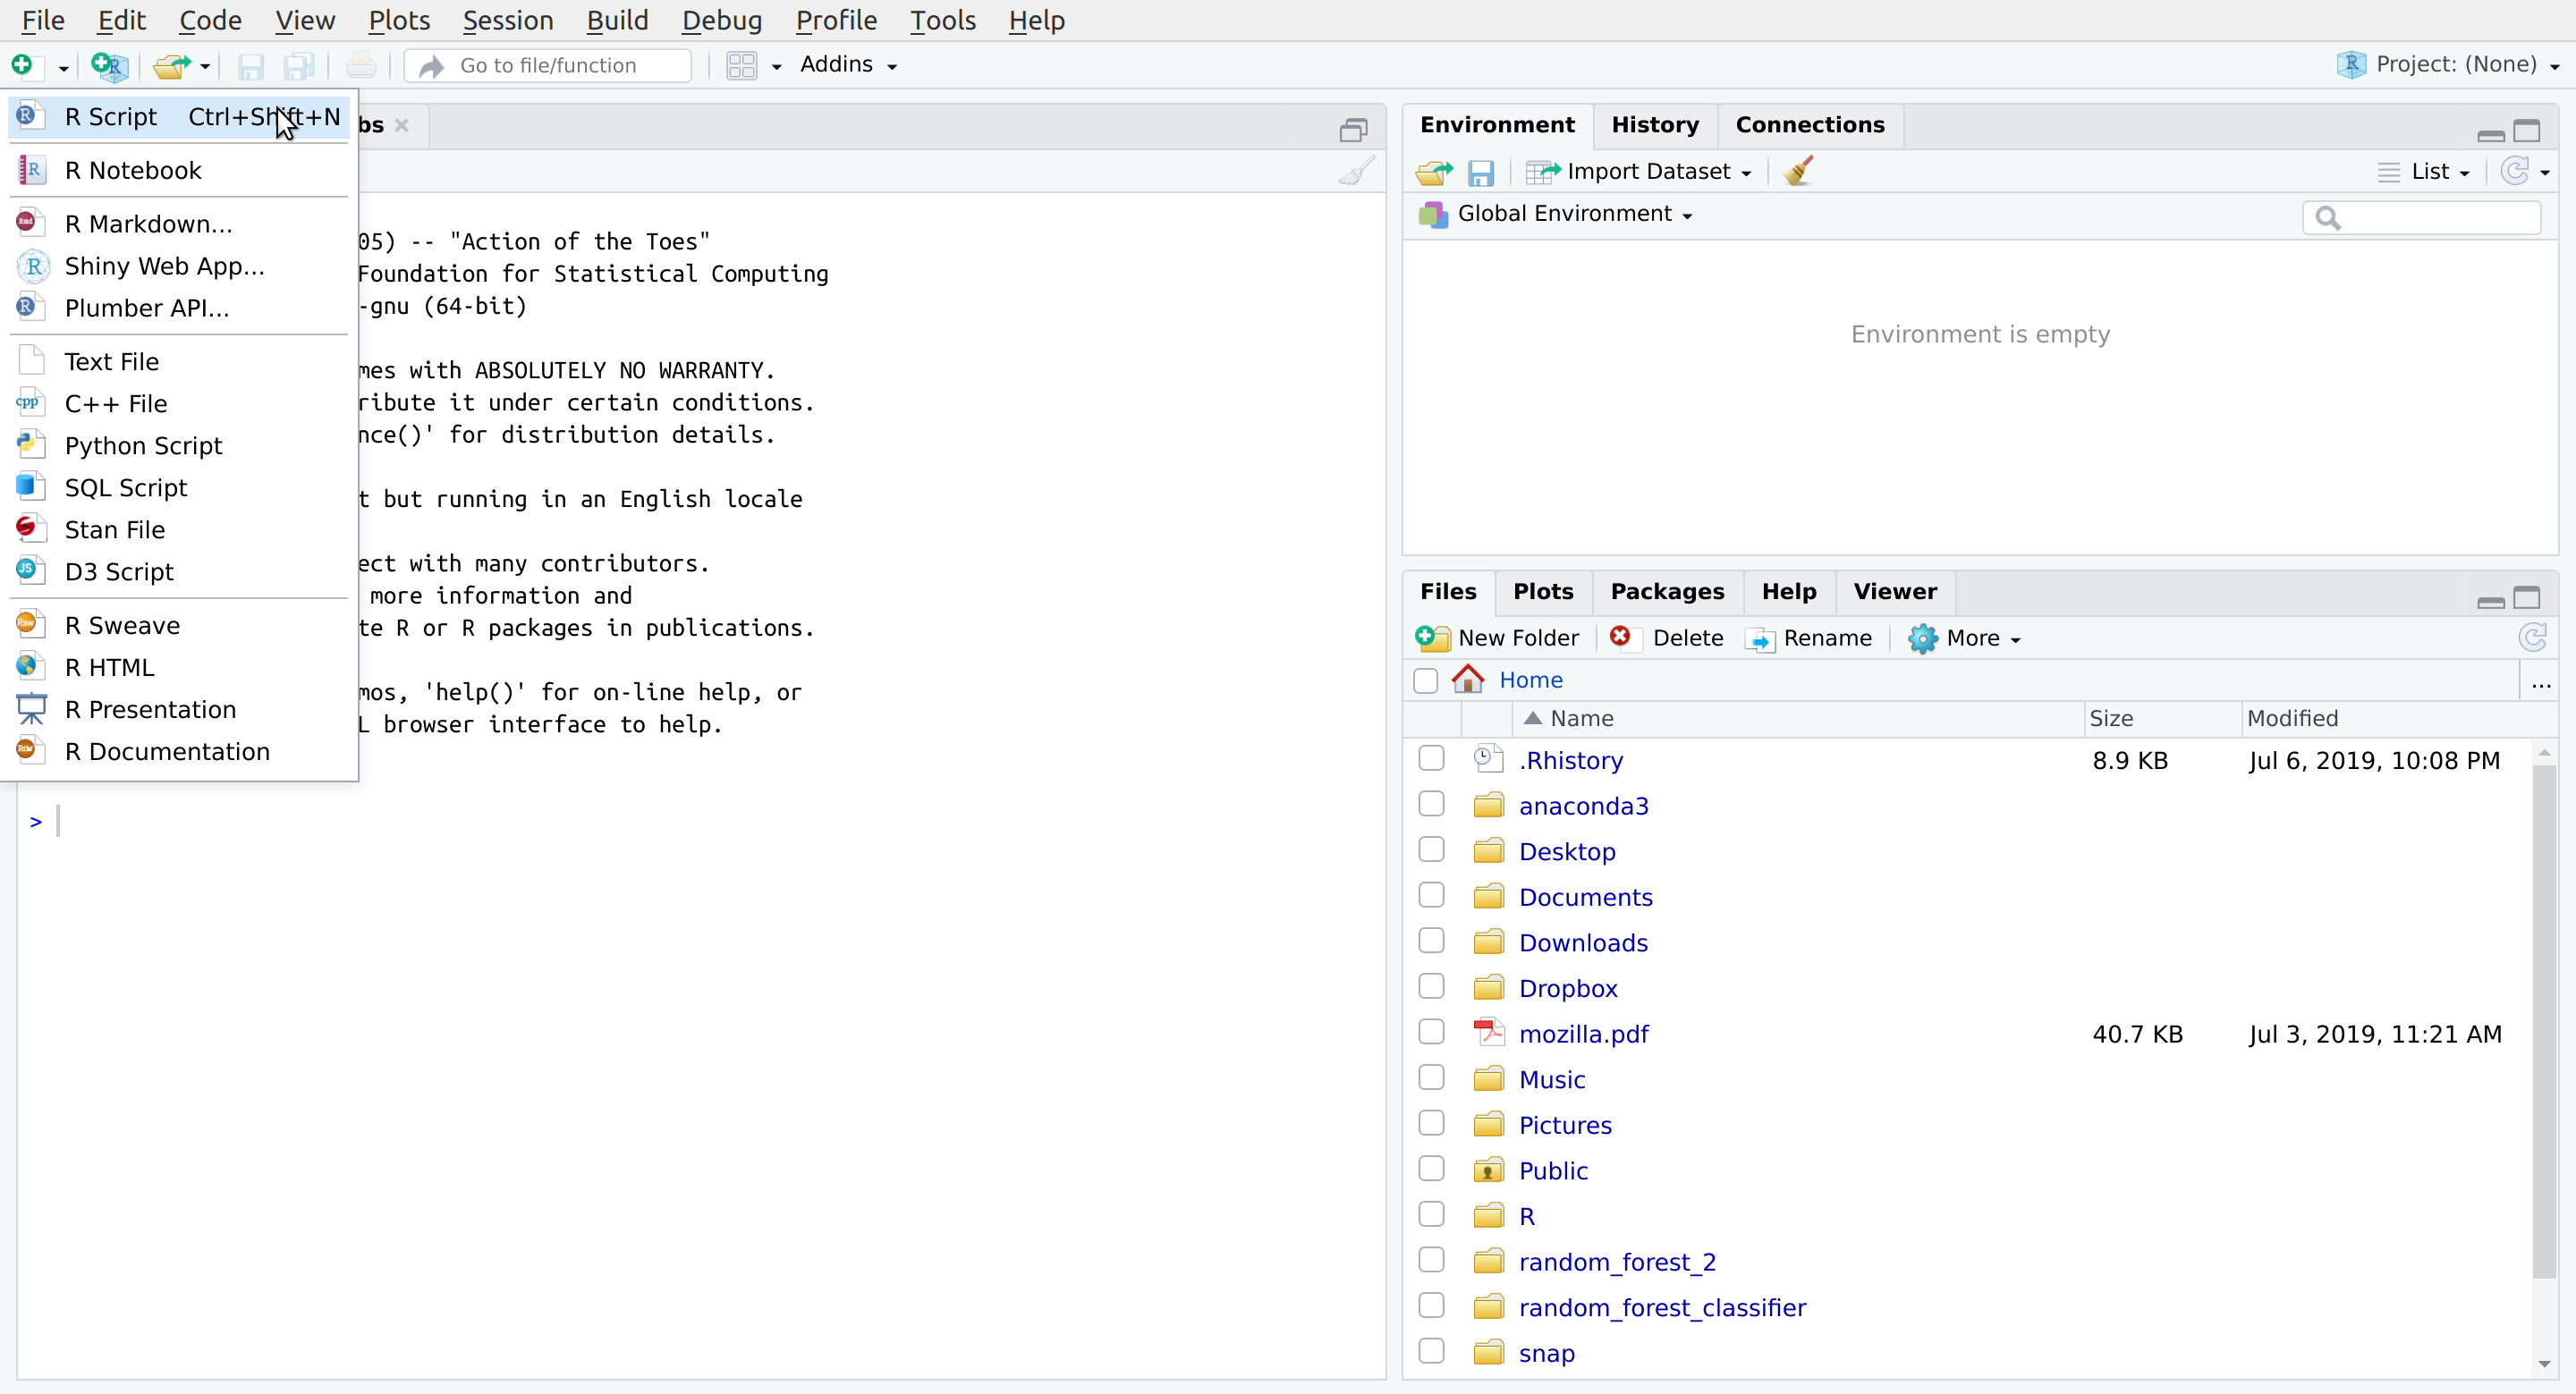
\includegraphics[width=40in]{images/RStudio2} \caption[Elige hoja+ para crear un nuevo archivo]{Elige hoja+ para crear un nuevo archivo}\label{fig:unnamed-chunk-10}
\end{figure}

Tendrás, entonces, 4 páneles como se ve a continuación:

\begin{figure}
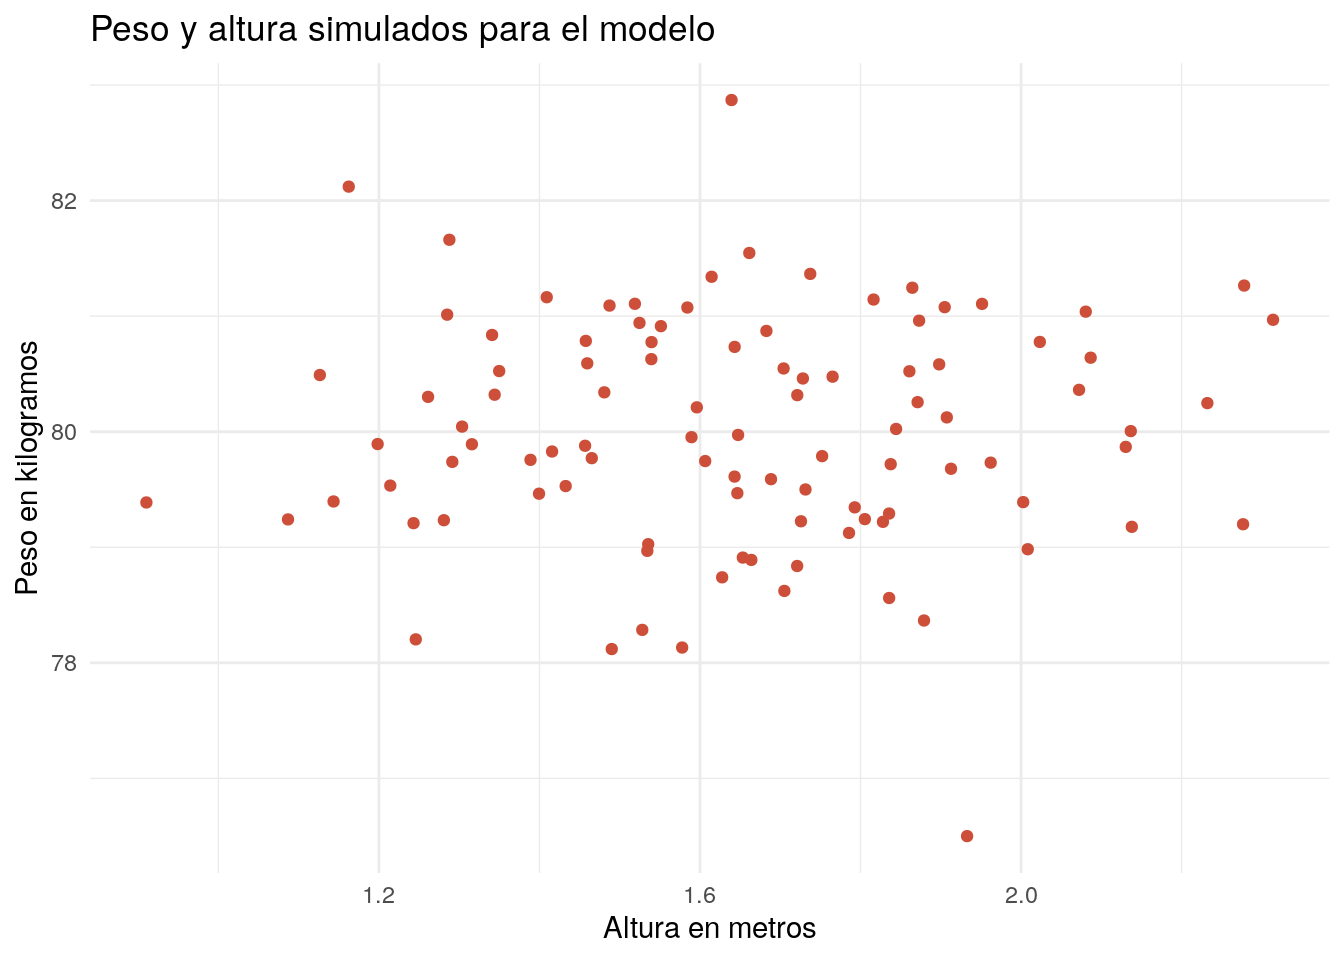
\includegraphics{Introducción_a_R_files/figure-latex/unnamed-chunk-11-1} \caption[RStudio <3]{RStudio <3}\label{fig:unnamed-chunk-11}
\end{figure}

\begin{enumerate}
\def\labelenumi{\arabic{enumi}.}
\tightlist
\item
  El primer panel (esquina inferior izquierda) es la \texttt{Consola}.
  Aquí es donde se ejecutan las acciones. Prueba escribir
  \texttt{2\ +\ 3} en él y presiona enter. Aparece el resultado de la
  suma. Definitivamente, \texttt{R} es la calculadora que más trabajo
  cuesta instalar.
\end{enumerate}

\begin{figure}
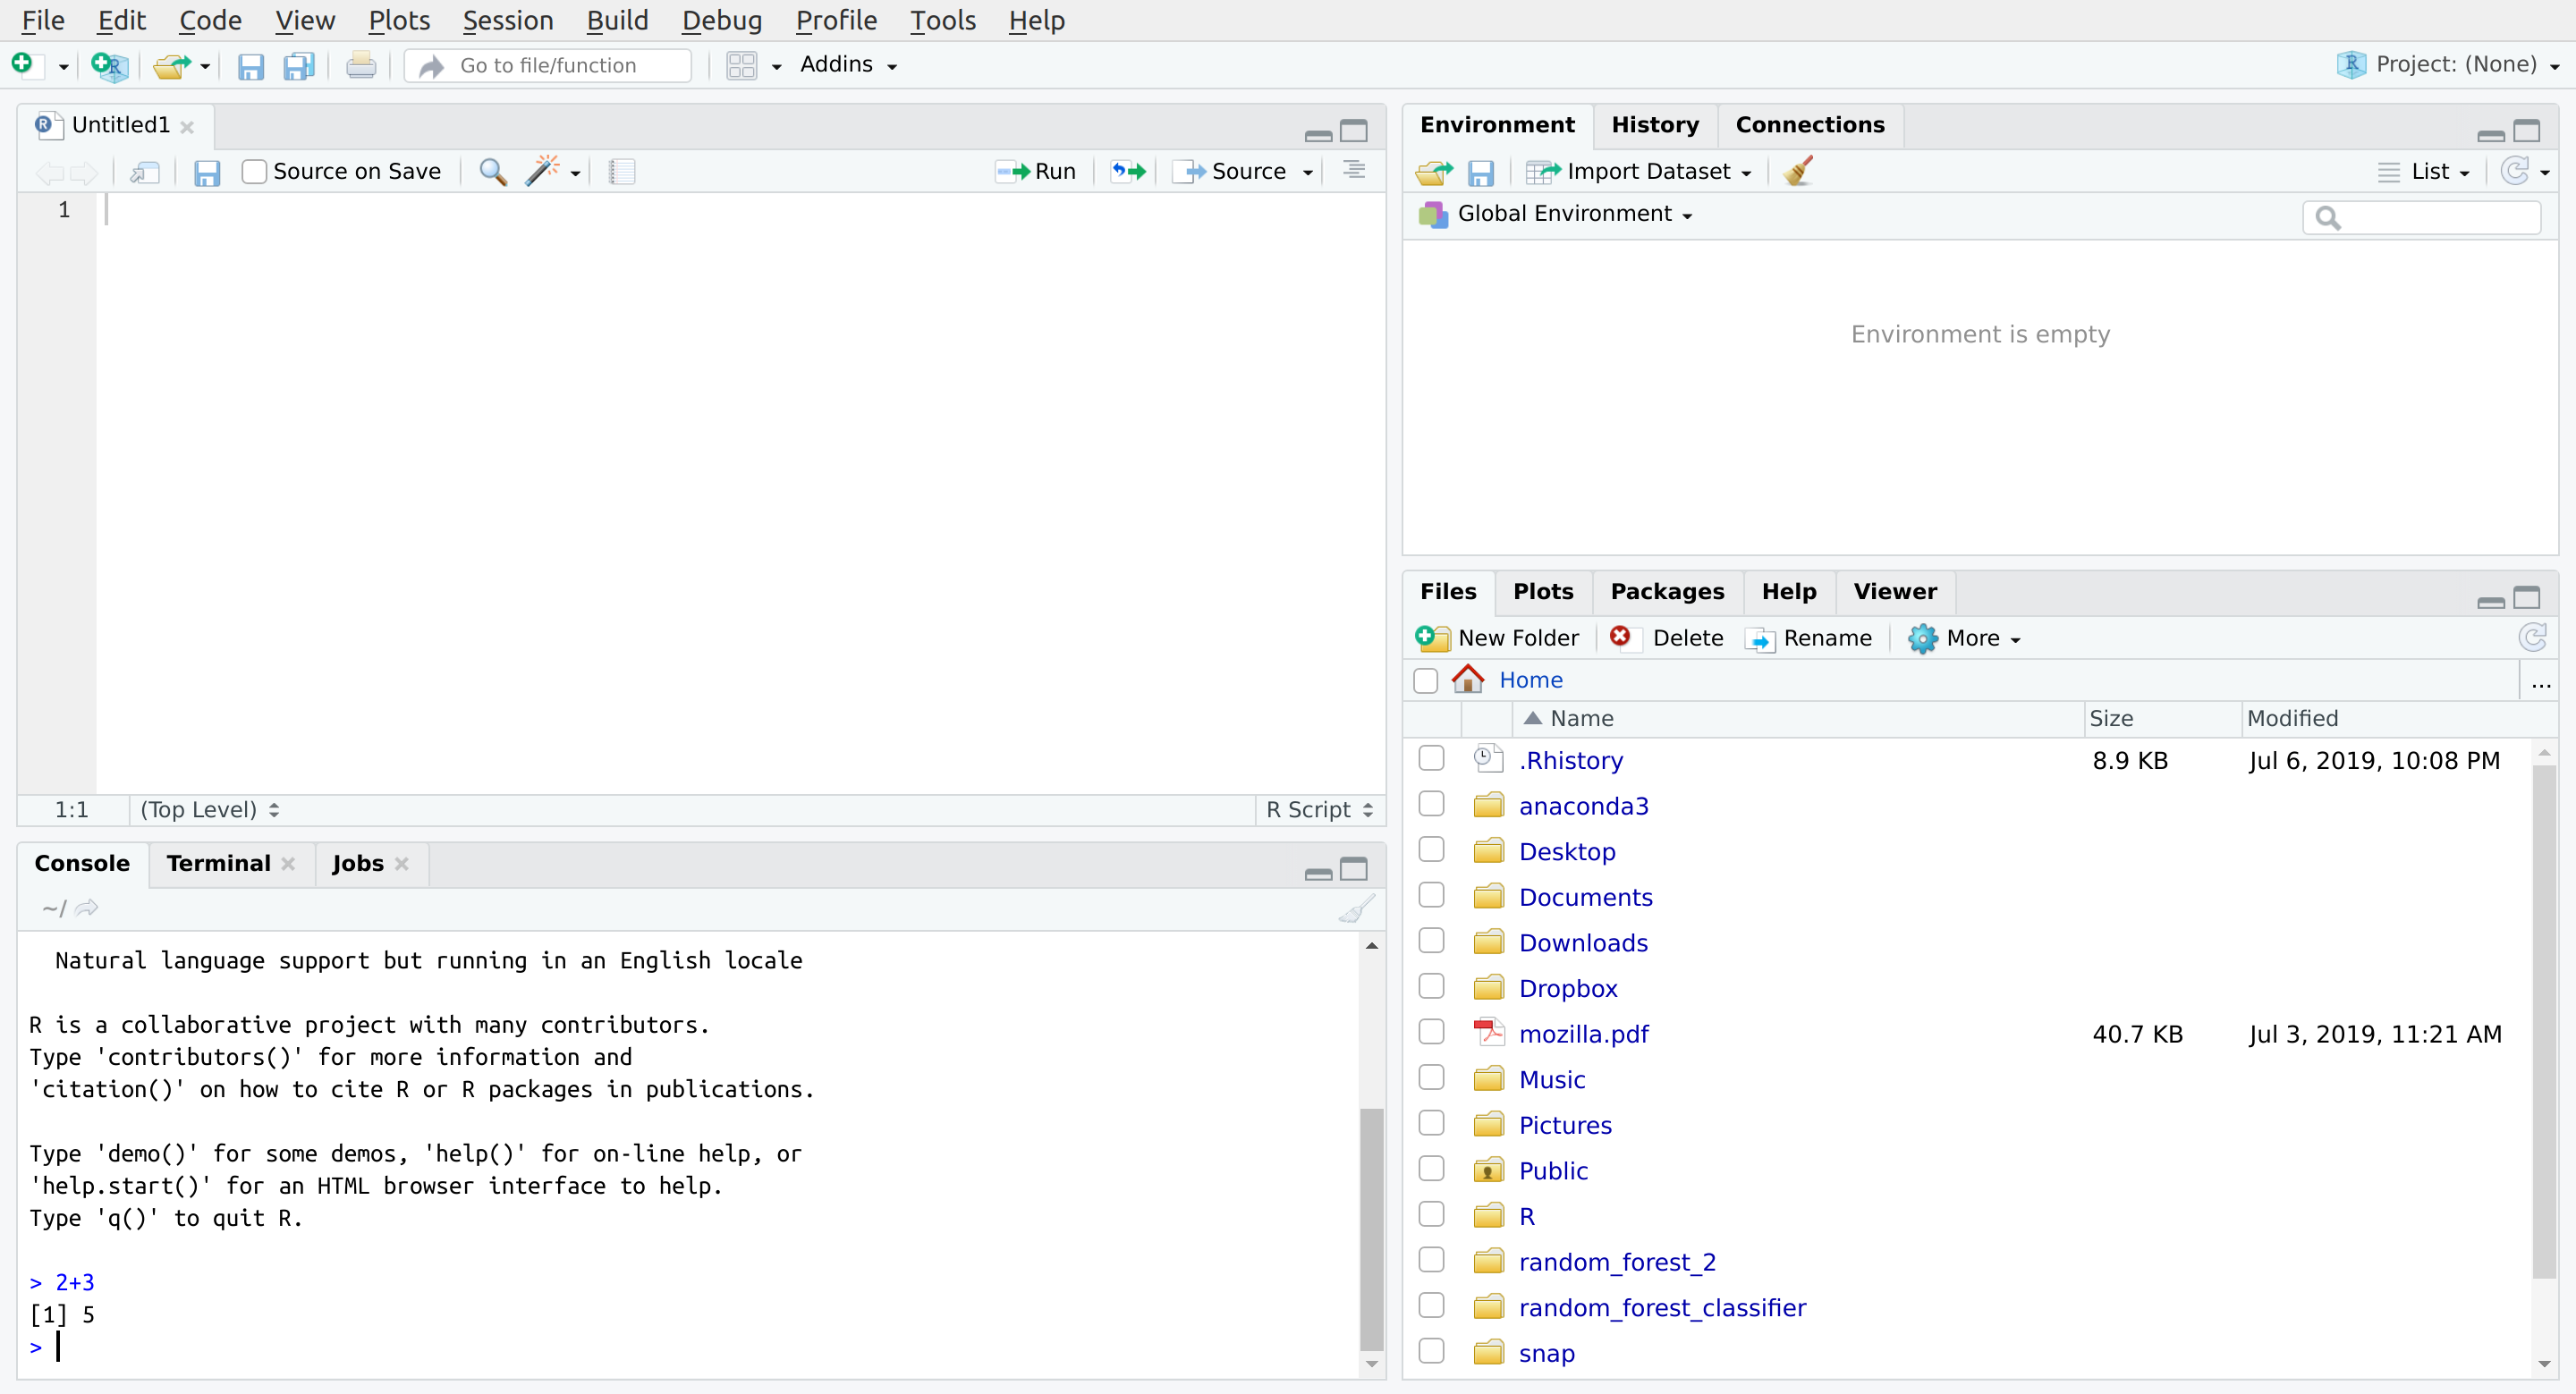
\includegraphics[width=40in]{images/RStudio4} \caption[La consola de `R` es la calculadora más difícil de instalar que existe]{La consola de `R` es la calculadora más difícil de instalar que existe.}\label{fig:unnamed-chunk-12}
\end{figure}

\begin{enumerate}
\def\labelenumi{\arabic{enumi}.}
\setcounter{enumi}{1}
\tightlist
\item
  El segundo panel (esquina superior izquierda) es el panel con el
  \texttt{Script}. Aquí se escribe el programa pero no \emph{se
  ejecuta}. Prueba escribir \texttt{10\ +\ 9}. ¿Ves que no pasa nada? Lo
  que acabas de hacer es crear un programa que, cuando se ejecute, hará
  la suma de \texttt{10\ +\ 9}. ¡Qué programa más aburrido! Sin embargo,
  no todo está perdido: presiona \texttt{CTRL+Enter} (\texttt{Cmd+Enter}
  en Mac) al final de la línea o bien da clic en \texttt{Run} y verás
  que, en la consola, aparece la instrucción y el resultado de la misma.
  El \texttt{Script} es una excelente fuente para tener un historial de
  lo que estás haciendo.
\end{enumerate}

\begin{figure}
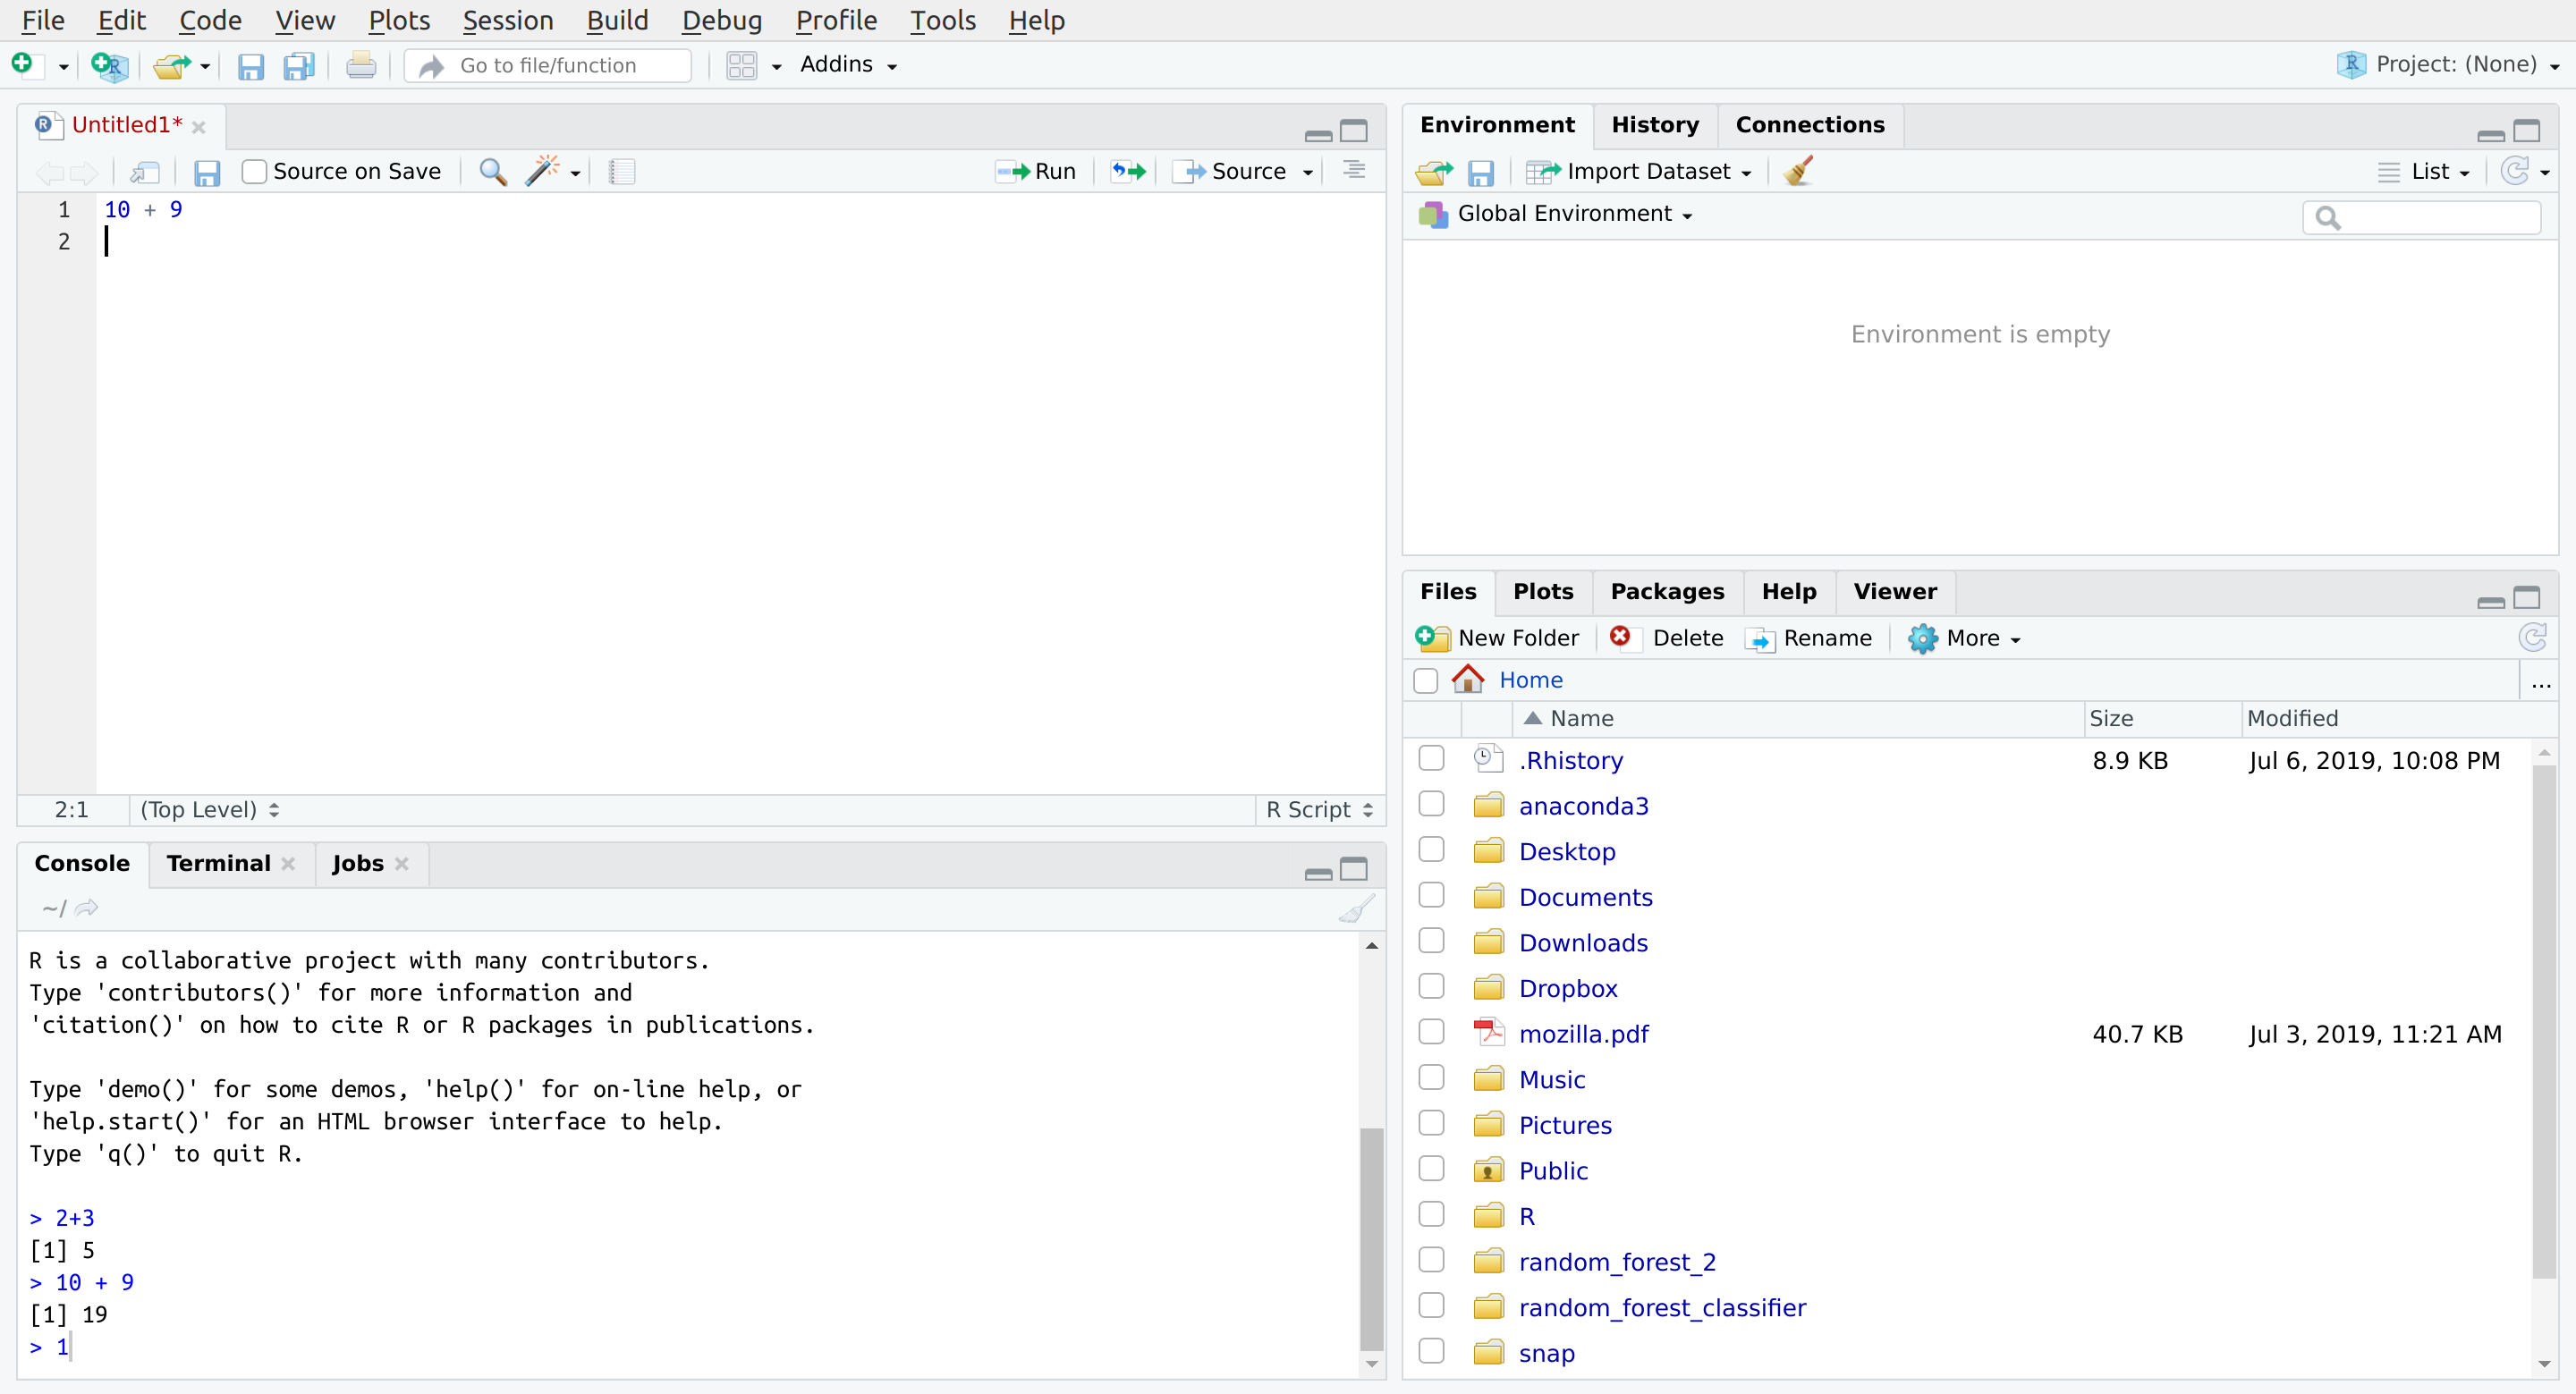
\includegraphics[width=40in]{images/RStudio5} \caption[El `Script` sirve para salvar las instrucciones en el orden en que las vas a ejecutar]{El `Script` sirve para salvar las instrucciones en el orden en que las vas a ejecutar.}\label{fig:unnamed-chunk-13}
\end{figure}

\begin{enumerate}
\def\labelenumi{\arabic{enumi}.}
\setcounter{enumi}{2}
\tightlist
\item
  El tercer panel contiene el ambiente. Aquí aparecerán las variables
  que vayamos creando. Por ahora, para poner un ejemplo, importaremos el
  archivo \texttt{Example1.csv} (con valores simulados) dando clic en
  \texttt{Import\ Dataset} y \texttt{From\ Text\ (base)}. Selecciona el
  archivo y elige las opciones en la ventana de previsualización que
  hagan que se vea bien. Nota que una vez realizada la importación
  aparece en el panel derecho \texttt{Example1.} Al dar clic podrás ver
  la base de datos. Las bases de datos y variables que utilices durante
  tus análisis aparecerán en esa sección.
\end{enumerate}

\begin{figure}
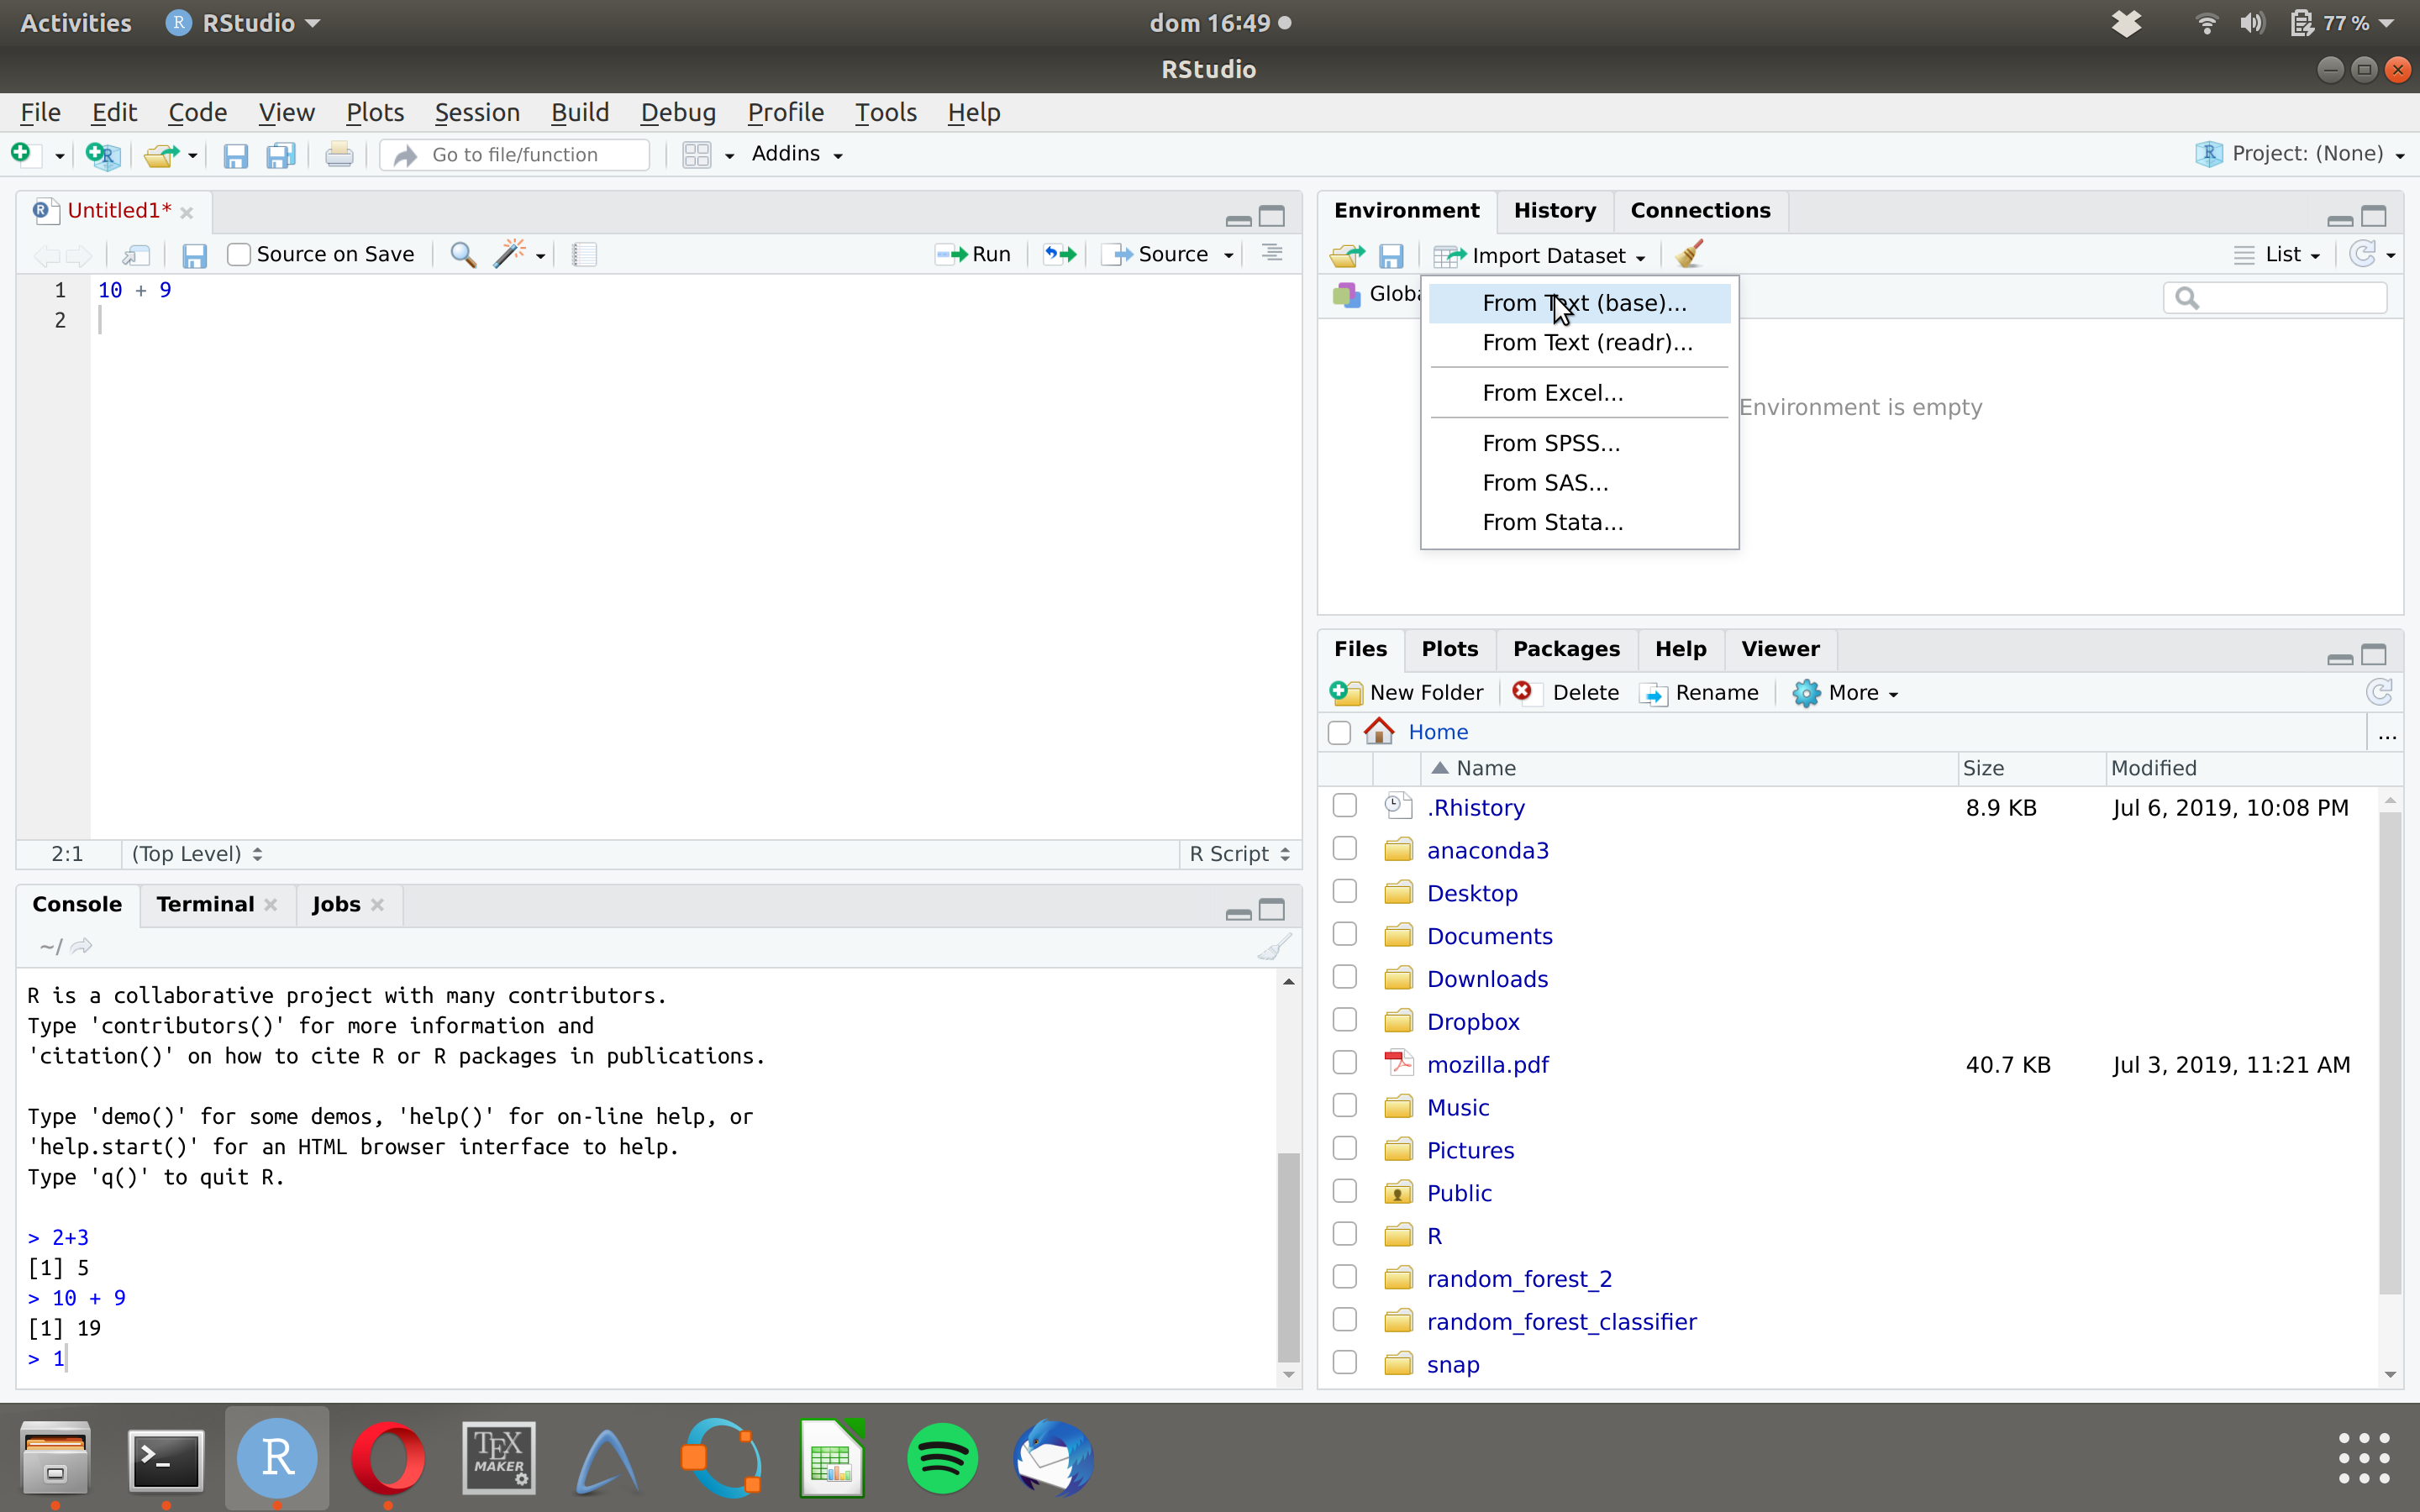
\includegraphics[width=40in]{images/RStudio6} \caption[El `Ambiente` muestra las variables (incluyendo bases de datos) que estás utilizando en este momento]{El `Ambiente` muestra las variables (incluyendo bases de datos) que estás utilizando en este momento. A diferencia de otros programas estadísticos (o sea `Stata`) en `R` es posible tener múltiples bases de datos abiertas a la vez.}\label{fig:unnamed-chunk-15}
\end{figure}

\begin{enumerate}
\def\labelenumi{\arabic{enumi}.}
\setcounter{enumi}{3}
\tightlist
\item
  Para entender mejor lo que ocurre en el último de los páneles, lo
  mejor es trabajar con nuestra base. Escribe en la consola
  \texttt{plot(Example1)} . En el cuarto pánel aparecerá una gráfica. El
  cuarto de los páneles para nosotros tendrá esa utilidad: mostrará las
  gráficas que hagamos así como la ayuda. Para ver la ayuda para las
  instrucciones de \texttt{R} puedes escribir \texttt{?}. Prueba teclear
  \texttt{?plot} en la consola. El signo de interrogación es un
  \texttt{help()} que muestra las instrucciones para usar una función.
\end{enumerate}

\begin{marginfigure}
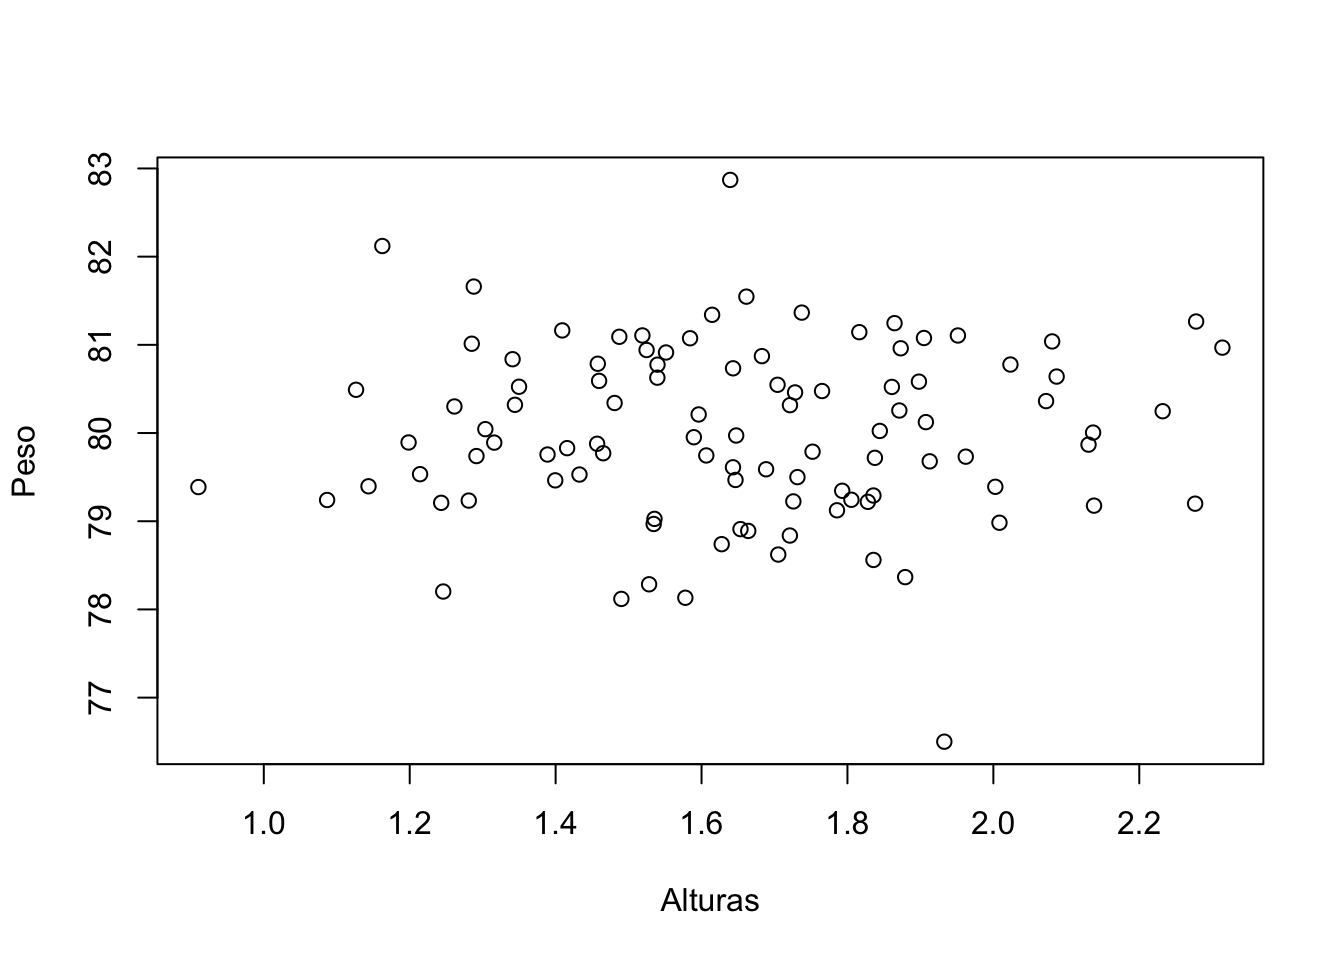
\includegraphics{Introducción_a_R_files/figure-latex/unnamed-chunk-16-1} \caption[La gráfica que aparece de hacer un `plot` de la base de datos de ejemplo]{La gráfica que aparece de hacer un `plot` de la base de datos de ejemplo.}\label{fig:unnamed-chunk-16}
\end{marginfigure}

\begin{figure}
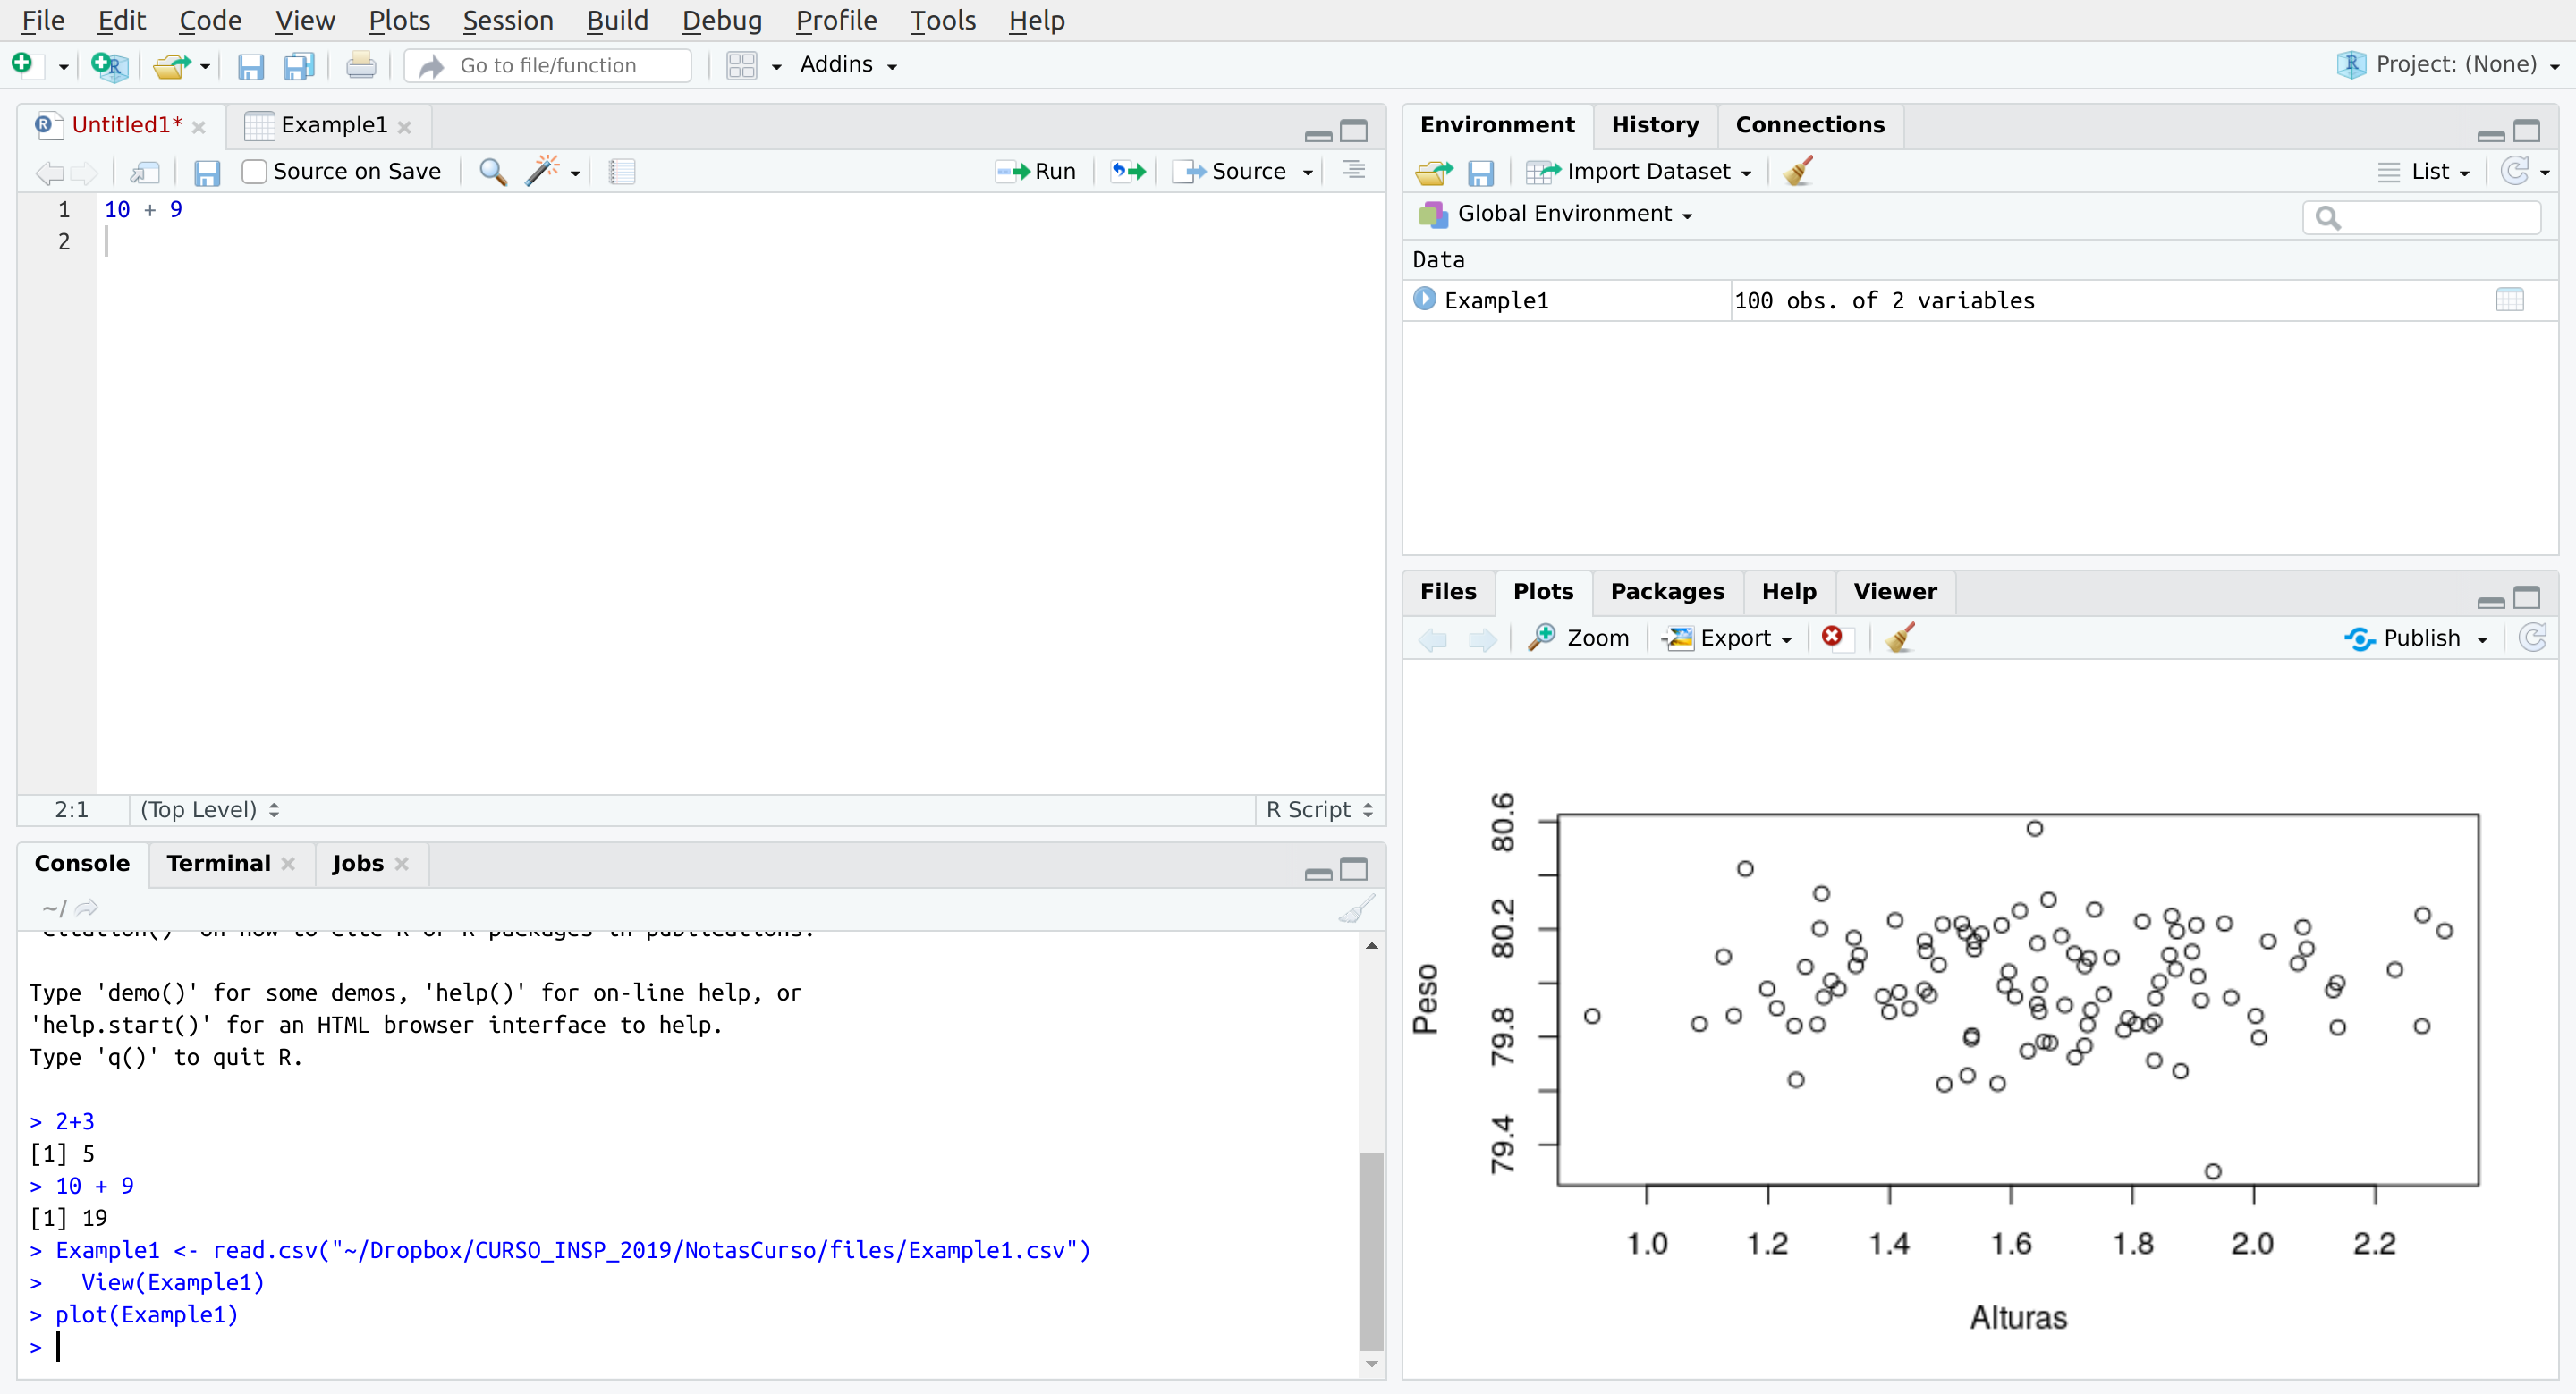
\includegraphics[width=40in]{images/RStudio7} \caption[El cuarto panel muestra respectivamente las gráficas y la ayuda]{El cuarto panel muestra respectivamente las gráficas y la ayuda.}\label{fig:unnamed-chunk-17}
\end{figure}

Mi sugerencia personal es que escribas todo lo que haces en el
\texttt{Script} y que sólo utilices la consola para verificar valores.
De esta manera podrás almacenar todas las instrucciones ejecutadas y
volver a ellas cuando se requieran. Por último te sugiero utilizar
\texttt{\#} gatos para comentar tu código. Así, el código anterior lo
podrías ver en la consola como:

\begin{Shaded}
\begin{Highlighting}[]
\CommentTok{\#Aquí pruebo cómo R hace las sumas}
\DecValTok{10} \SpecialCharTok{+} \DecValTok{9}
\end{Highlighting}
\end{Shaded}

\href{https://www.freecodecamp.org/news/code-comments-the-good-the-bad-and-the-ugly-be9cc65fbf83/}{Comenta}.
\href{https://www.c-sharpcorner.com/blogs/why-comments-are-important-while-writing-a-code}{Comenta}.
\href{https://blog.codinghorror.com/code-tells-you-how-comments-tell-you-why/}{Comenta,
por favor}. Tu ser del futuro que regrese a sus archivos de \texttt{R}
un mes después de haberlos hecho te lo agradecerá (y tu profe también).

Finalmente y como aclaración para estas notas, el código de \texttt{R}
aparece como:

\begin{Shaded}
\begin{Highlighting}[]
\CommentTok{\#Esto es código de R}
\DecValTok{7} \SpecialCharTok{{-}} \DecValTok{2}
\end{Highlighting}
\end{Shaded}

Mientras que los resultados de evaluar en \texttt{R} se ven con
\texttt{\#}:

\begin{verbatim}
## [1] 5
\end{verbatim}

Así, la evaluación con su resultado se ve de la siguiente forma:

\begin{Shaded}
\begin{Highlighting}[]
\CommentTok{\#Esto es código de R}
\DecValTok{7} \SpecialCharTok{{-}} \DecValTok{2}
\end{Highlighting}
\end{Shaded}

\begin{verbatim}
## [1] 5
\end{verbatim}

\hypertarget{primeros-pasos-con-r}{%
\chapter{\texorpdfstring{Primeros pasos con
\texttt{R}}{Primeros pasos con R}}\label{primeros-pasos-con-r}}

\hypertarget{cuxe1lculos-numuxe9ricos}{%
\section{Cálculos numéricos}\label{cuxe1lculos-numuxe9ricos}}

\texttt{R} sirve como calculadora para las operaciones usuales. En él
puedes hacer sumas,

\begin{Shaded}
\begin{Highlighting}[]
\CommentTok{\#Esto es una suma en R}
\DecValTok{12} \SpecialCharTok{+} \DecValTok{31}
\end{Highlighting}
\end{Shaded}

\begin{verbatim}
## [1] 43
\end{verbatim}

\begin{marginfigure}
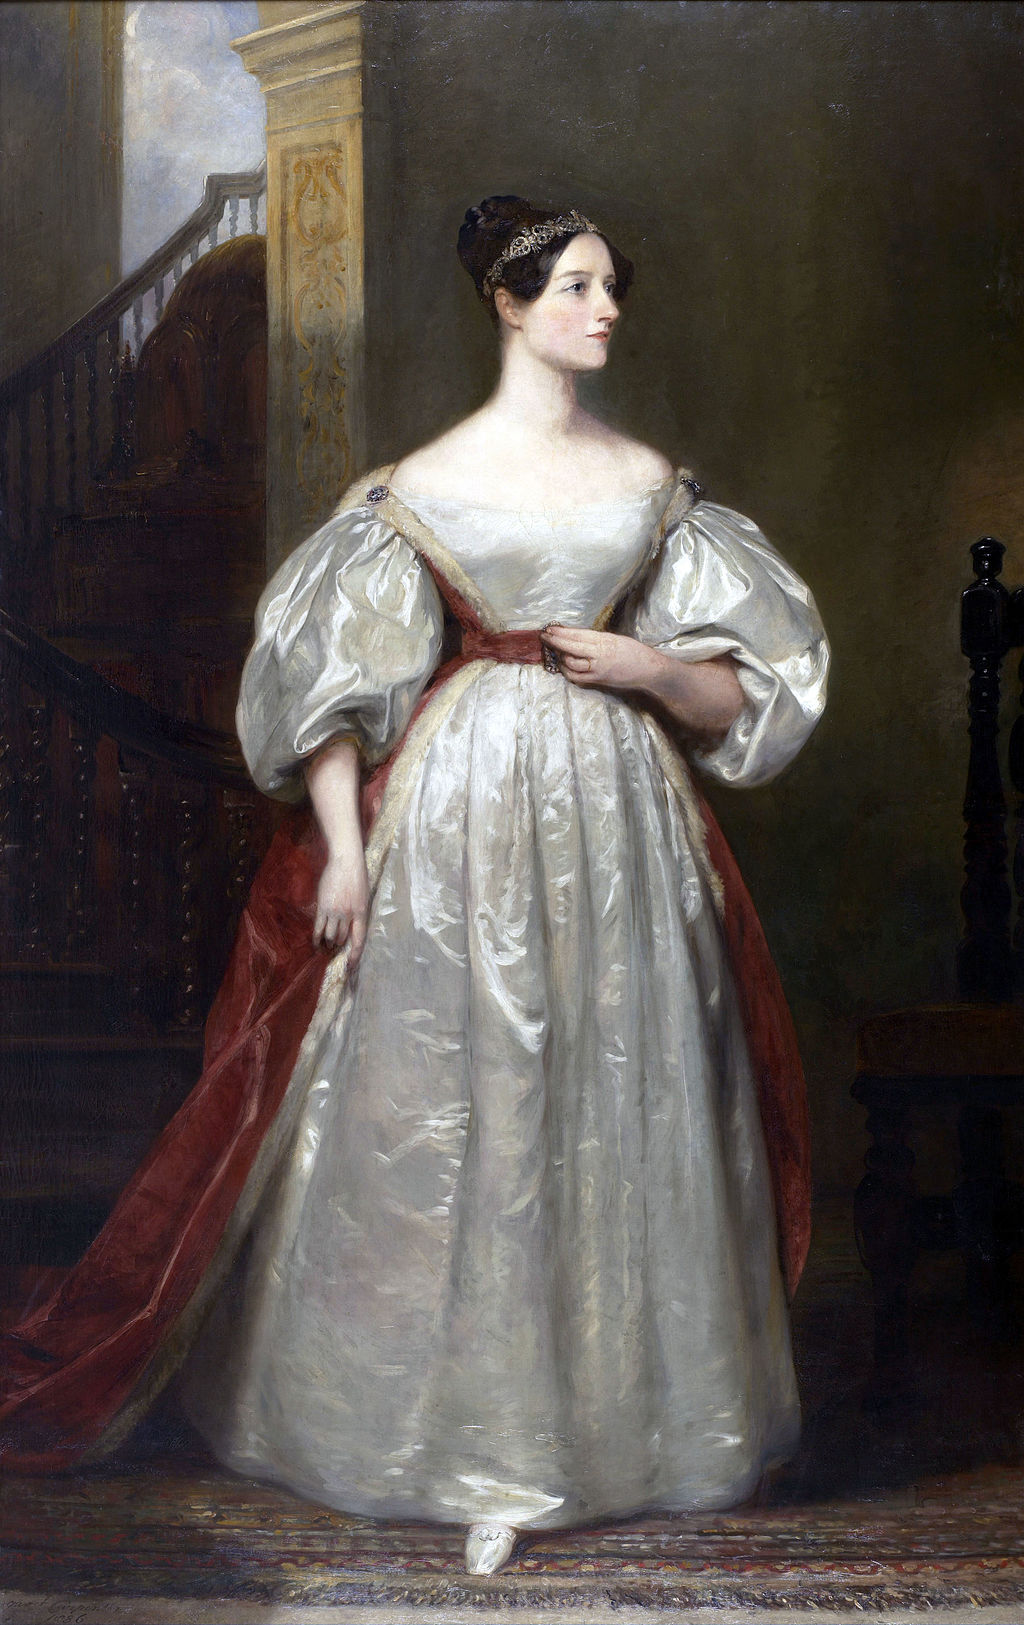
\includegraphics[width=14.22in]{images/ada_lovelace} \caption[Ada Lovelace (1815-1852), la primera en diseñar un algoritmo computacional ¡y sin tener computadoras!]{Ada Lovelace (1815-1852), la primera en diseñar un algoritmo computacional ¡y sin tener computadoras!}\label{fig:unnamed-chunk-23}
\end{marginfigure}

restas,

\begin{Shaded}
\begin{Highlighting}[]
\CommentTok{\#Esto es una resta en R}
\DecValTok{3} \SpecialCharTok{{-}} \DecValTok{4}
\end{Highlighting}
\end{Shaded}

\begin{verbatim}
## [1] -1
\end{verbatim}

multiplicaciones,

\begin{Shaded}
\begin{Highlighting}[]
\CommentTok{\#Esto es una multiplicación en R}
\DecValTok{7}\SpecialCharTok{*}\DecValTok{8}
\end{Highlighting}
\end{Shaded}

\begin{verbatim}
## [1] 56
\end{verbatim}

divisiones,

\begin{Shaded}
\begin{Highlighting}[]
\CommentTok{\#Esto es una división en R}
\DecValTok{4}\SpecialCharTok{/}\DecValTok{2}
\end{Highlighting}
\end{Shaded}

\begin{verbatim}
## [1] 2
\end{verbatim}

sacar logaritmos naturales \(\ln\),

\begin{Shaded}
\begin{Highlighting}[]
\CommentTok{\#Para sacar logaritmo usas el comando log}
\FunctionTok{log}\NormalTok{(}\DecValTok{100}\NormalTok{)}
\end{Highlighting}
\end{Shaded}

\begin{verbatim}
## [1] 4.60517
\end{verbatim}

o bien logaritmos en cualquier base,\footnote{Recuerda que un logaritmo
  base \(a\) te dice a qué potencia \(b\) tuve que elevar \(a\) para
  llegar a \(b\). Por ejemplo \(\log_{10}(100) = 2\) te dice que para
  llegar al \(100\) tuviste que hacer \(10^2\).}

\begin{Shaded}
\begin{Highlighting}[]
\CommentTok{\#Puedes especificar la base del logaritmo con base }
\FunctionTok{log}\NormalTok{(}\DecValTok{100}\NormalTok{, }\AttributeTok{base =} \DecValTok{10}\NormalTok{)}
\end{Highlighting}
\end{Shaded}

\begin{verbatim}
## [1] 2
\end{verbatim}

también puedes elevar a una potencia (por ejemplo hacer \(6^3\)),

\begin{Shaded}
\begin{Highlighting}[]
\CommentTok{\#Así se calculan potencias}
\DecValTok{6}\SpecialCharTok{\^{}}\DecValTok{3}
\end{Highlighting}
\end{Shaded}

\begin{verbatim}
## [1] 216
\end{verbatim}

calcular la exponencial \(e\),

\begin{Shaded}
\begin{Highlighting}[]
\CommentTok{\#Para exponenciales puedes usar exp}
\FunctionTok{exp}\NormalTok{(}\DecValTok{1}\NormalTok{)}
\end{Highlighting}
\end{Shaded}

\begin{verbatim}
## [1] 2.718282
\end{verbatim}

o bien exponenciar cualquier variable \(e^{-3}\),

\begin{Shaded}
\begin{Highlighting}[]
\CommentTok{\#O bien exponenciales específicas, e\^{}{-}3}
\FunctionTok{exp}\NormalTok{(}\SpecialCharTok{{-}}\DecValTok{3}\NormalTok{)}
\end{Highlighting}
\end{Shaded}

\begin{verbatim}
## [1] 0.04978707
\end{verbatim}

también puedes usar el número \(\pi\).

\begin{Shaded}
\begin{Highlighting}[]
\CommentTok{\#Cálculo de pi}
\NormalTok{pi}
\end{Highlighting}
\end{Shaded}

\begin{verbatim}
## [1] 3.141593
\end{verbatim}

No olvides que \texttt{R} usa el orden de las operaciones de
matemáticas. Siempre es de izquierda a derecha con las siguientes
excepciones:

\begin{enumerate}
\def\labelenumi{\arabic{enumi}.}
\item
  Primero se evalúa lo que está entre paréntesis.
\item
  En segundo lugar se calculan potencias.
\item
  Lo tercero en evaluarse son multiplicaciones y divisiones.
\item
  Finalmente, se realizan sumas y restas.
\end{enumerate}

Por ejemplo, en la siguiente ecuación \[
2 - 2 \cdot \frac{(3^4 - 9)}{(5 + 4)}
\] se resuelven primero los paréntesis \((3^4 - 9) = 81 - 9 = 72\) y
\((5 + 4) = 9\); luego se resuelve la división: \(\frac{72}{9}=8\), se
multiplica por el \(2\): \(2 \cdot 8\) y finalmente se hace la resta:
\(2-8 = -6\).

\hypertarget{ejercicio}{%
\section{Ejercicio}\label{ejercicio}}

Determina, sin evaluar, los resultados de los siguientes segmentos de
código:

\begin{Shaded}
\begin{Highlighting}[]
\CommentTok{\#Primer ejercicio }
\NormalTok{(}\DecValTok{9} \SpecialCharTok{{-}} \DecValTok{3}\NormalTok{)}\SpecialCharTok{\^{}}\DecValTok{2} \SpecialCharTok{*}\NormalTok{ (}\DecValTok{2} \SpecialCharTok{{-}} \DecValTok{1}\NormalTok{) }\SpecialCharTok{{-}} \DecValTok{6}
\end{Highlighting}
\end{Shaded}

\begin{Shaded}
\begin{Highlighting}[]
\CommentTok{\#Segundo ejercicio }
\DecValTok{6} \SpecialCharTok{*} \DecValTok{2} \SpecialCharTok{/}\NormalTok{ (}\DecValTok{7} \SpecialCharTok{{-}} \DecValTok{3}\NormalTok{) }\SpecialCharTok{*} \DecValTok{5}
\end{Highlighting}
\end{Shaded}

\begin{Shaded}
\begin{Highlighting}[]
\CommentTok{\#Tercer ejercicio }
\DecValTok{2} \SpecialCharTok{*} \DecValTok{3} \SpecialCharTok{\^{}} \DecValTok{2} \SpecialCharTok{*} \DecValTok{2} \SpecialCharTok{/}\NormalTok{ (}\DecValTok{5} \SpecialCharTok{{-}} \DecValTok{4}\NormalTok{) }\SpecialCharTok{*} \DecValTok{1} \SpecialCharTok{/} \DecValTok{10} 
\end{Highlighting}
\end{Shaded}

Evalúa para comprobar tu respuesta.

\hypertarget{ejercicio-1}{%
\section{Ejercicio}\label{ejercicio-1}}

Calcula el área y el perímetro de un círculo de radio 5. Recuerda que la
fórmula del área es \(\pi \cdot r^2\) donde \(r\) es el radio; mientras
que la del perímetro es: \(\pi \cdot d\) donde \(d\) es el díametro (=
dos veces el radio).

\hypertarget{respuestas}{%
\subsection{Respuestas}\label{respuestas}}

\begin{verbatim}
## Área = 78.5398163397448
\end{verbatim}

\begin{verbatim}
## Perímetro = 31.4159265358979
\end{verbatim}

\hypertarget{variables}{%
\section{Variables}\label{variables}}

\texttt{R} es un programa orientado a objetos; esto quiere decir que
\texttt{R} almacena la información en un conjunto de variables que
pueden tener diferentes \texttt{clases} y opera con ellos según su
clase. Por ejemplo, un conjunto de caracteres, entre comillas, es un
\texttt{Character} (\texttt{R} lo piensa como texto)

\begin{Shaded}
\begin{Highlighting}[]
\CommentTok{\#Un conjunto de caracteres es un char}
\StringTok{"Hola"}
\end{Highlighting}
\end{Shaded}

\begin{verbatim}
## [1] "Hola"
\end{verbatim}

Un número (por ejemplo \texttt{2} tiene clase
\texttt{numeric})\footnote{Puede ser \texttt{float}, \texttt{int},
  \texttt{double} pero no nos preocuparemos por eso.}. Hay que tener
mucho cuidado con combinar floats con \texttt{Strings}:

\begin{Shaded}
\begin{Highlighting}[]
\CommentTok{\#Código que sí funciona porque ambos son números}
\DecValTok{2} \SpecialCharTok{+} \DecValTok{4} 
\end{Highlighting}
\end{Shaded}

\begin{verbatim}
## [1] 6
\end{verbatim}

\begin{marginfigure}
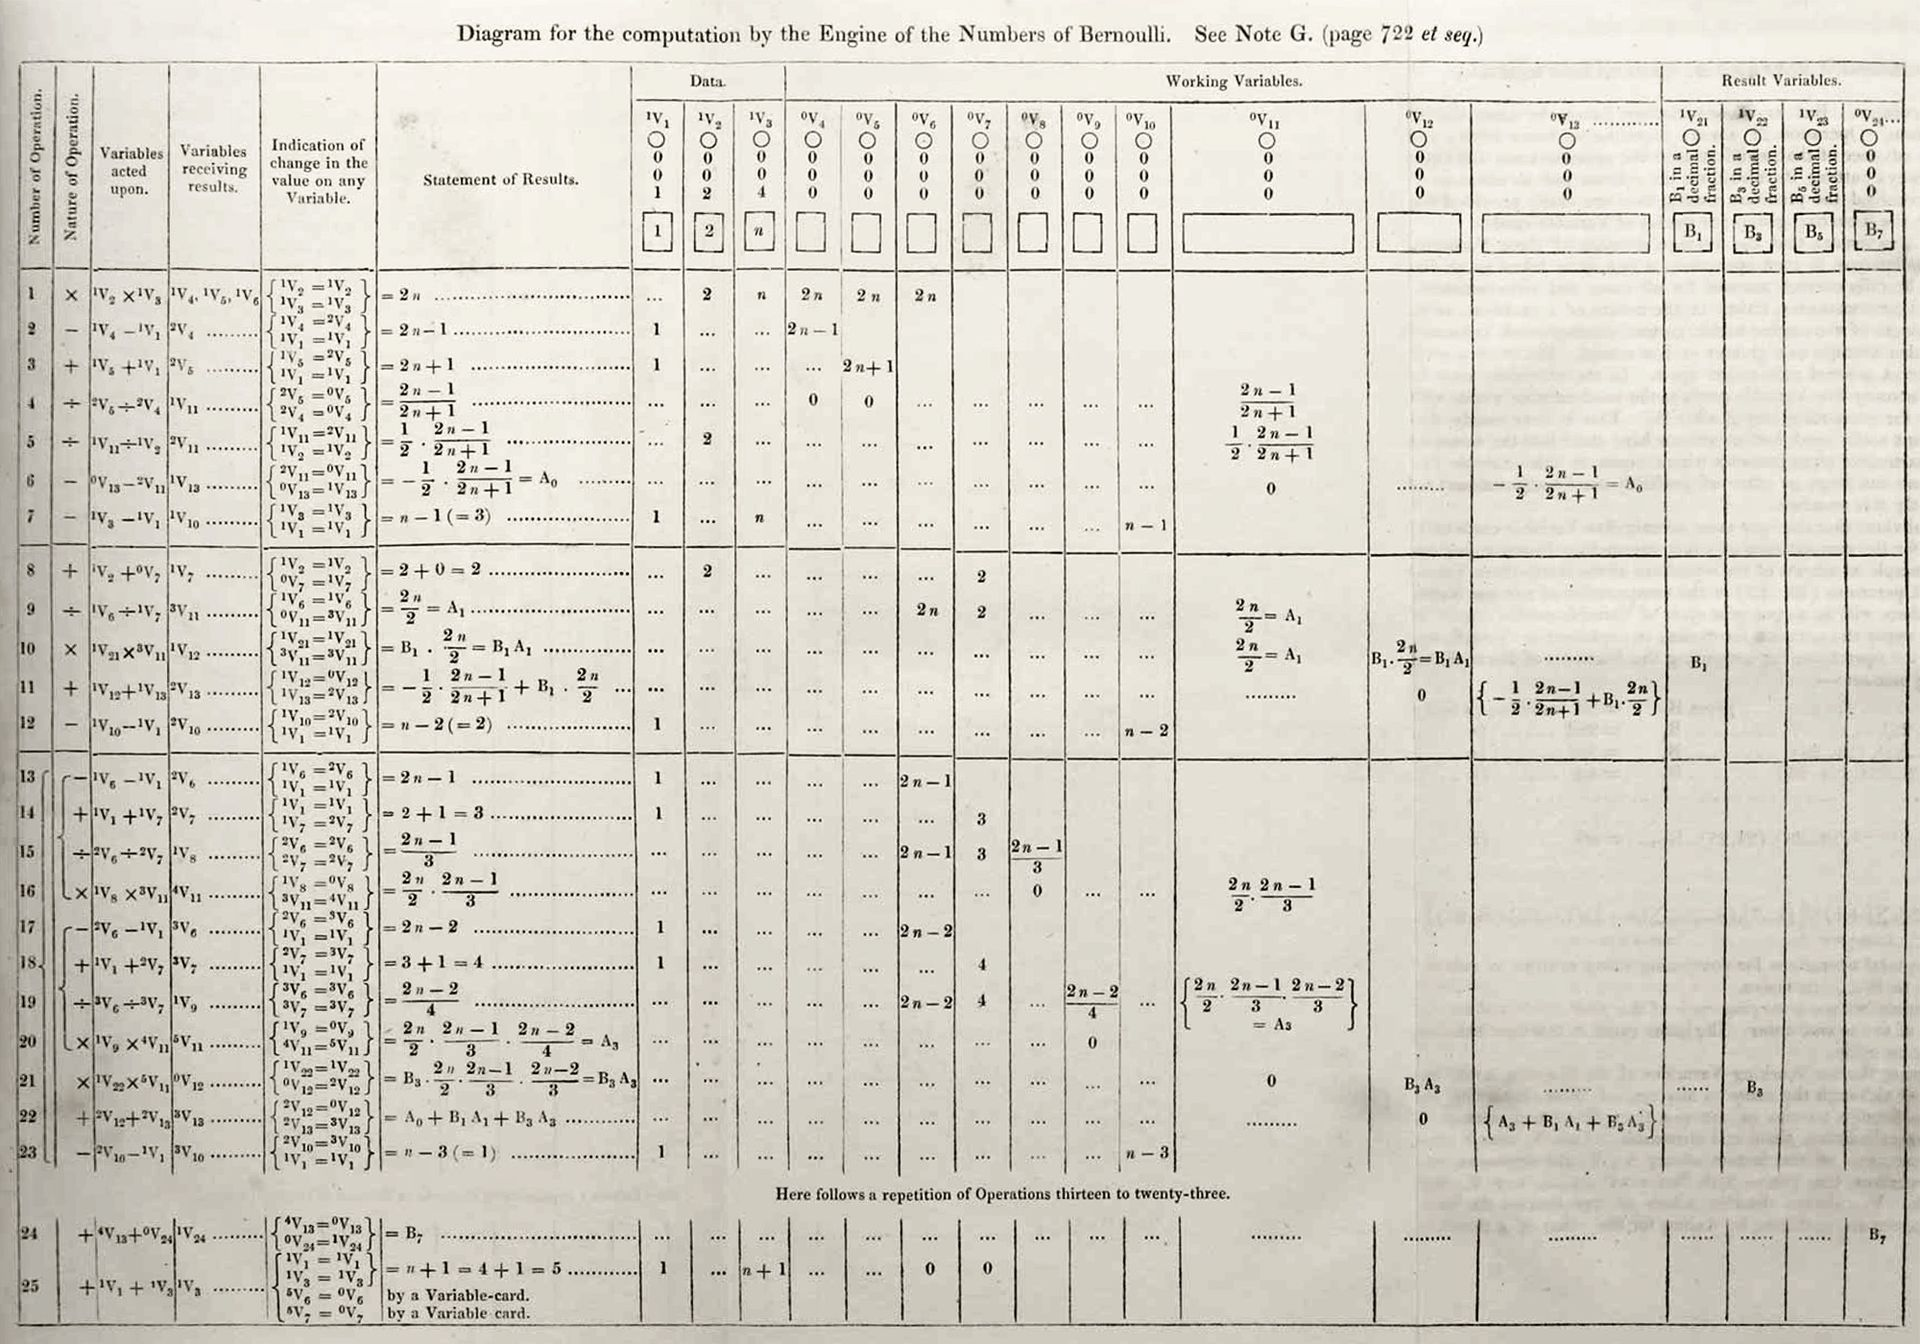
\includegraphics[width=26.67in]{images/algorithm_lovelace} \caption[El algoritmo diseñado por Ada Lovelace]{El algoritmo diseñado por Ada Lovelace.}\label{fig:unnamed-chunk-39}
\end{marginfigure}

\begin{Shaded}
\begin{Highlighting}[]
\CommentTok{\#Código que no funciona porque uno es caracter}
\DecValTok{2} \SpecialCharTok{+} \StringTok{"4"} 
\end{Highlighting}
\end{Shaded}

\begin{verbatim}
## Error in 2 + "4": non-numeric argument to binary operator
\end{verbatim}

Si lo piensas, este último error ¡tiene todo el sentido! no puedes sumar
un número a un texto. ¿O qué significaría
\texttt{\textquotesingle{}Felices\textquotesingle{}\ *\ 4} ?

La magia de \texttt{R} comienza con que puedes almacenar valores en
variables. Por ejemplo, podemos asignar un valor a una variable:

\begin{Shaded}
\begin{Highlighting}[]
\CommentTok{\#Asignamos x = 10}
\NormalTok{x }\OtherTok{\textless{}{-}} \DecValTok{10}
\end{Highlighting}
\end{Shaded}

Hay dos formas de asignar valores, una es con la flecha de asignación
\(\leftarrow\) y otra con el signo de igual:

\begin{Shaded}
\begin{Highlighting}[]
\CommentTok{\#Podemos asignar valores con el signo de =}
\NormalTok{y }\OtherTok{=} \DecValTok{6}
\end{Highlighting}
\end{Shaded}

Nota que, cuando realizamos operaciones, la asignación es la última que
se realiza:

\begin{Shaded}
\begin{Highlighting}[]
\CommentTok{\#Aquí z = 106}
\NormalTok{z }\OtherTok{\textless{}{-}}\NormalTok{ y }\SpecialCharTok{+}\NormalTok{ x}\SpecialCharTok{\^{}}\DecValTok{2}
\end{Highlighting}
\end{Shaded}

Los valores que fueron asignados en las variables, \texttt{R} los
recuerda y es posible calcular con ellos:

\begin{Shaded}
\begin{Highlighting}[]
\CommentTok{\#Podemos realizar una suma}
\NormalTok{x }\SpecialCharTok{+}\NormalTok{ y}
\end{Highlighting}
\end{Shaded}

\begin{verbatim}
## [1] 16
\end{verbatim}

\begin{Shaded}
\begin{Highlighting}[]
\CommentTok{\#O bien podemos realizar una multiplicación}
\DecValTok{3}\SpecialCharTok{*}\NormalTok{y }\SpecialCharTok{{-}}\NormalTok{ x}
\end{Highlighting}
\end{Shaded}

\begin{verbatim}
## [1] 8
\end{verbatim}

Podemos preguntarnos por el valor de las variables numéricas mediante
los operadores \texttt{==} (sí, son dos iguales), \texttt{!=} (que es un
\(\neq\)) \texttt{\textgreater{}}, \texttt{\textgreater{}=},
\texttt{\textless{}=} y \texttt{\textless{}}:

\begin{Shaded}
\begin{Highlighting}[]
\CommentTok{\#Podemos preguntarnos si x vale 4}
\NormalTok{x }\SpecialCharTok{==} \DecValTok{4}
\end{Highlighting}
\end{Shaded}

\begin{verbatim}
## [1] FALSE
\end{verbatim}

\begin{marginfigure}
El operador de asignación también se puede utilizar al revés
\(2 \rightarrow x\) pero no lo hagas, por favor.
\end{marginfigure}

Nota que no estamos asignando el valor de \texttt{x}:

\begin{Shaded}
\begin{Highlighting}[]
\NormalTok{x}
\end{Highlighting}
\end{Shaded}

\begin{verbatim}
## [1] 10
\end{verbatim}

Podemos preguntarnos por diferencia:

\begin{Shaded}
\begin{Highlighting}[]
\NormalTok{x }\SpecialCharTok{!=} \DecValTok{4} 
\end{Highlighting}
\end{Shaded}

\begin{verbatim}
## [1] TRUE
\end{verbatim}

Así como por mayores, menores incluyendo posibles igualdades
(\emph{i.e.} los casos \(\geq\) y \(\leq\))

\begin{Shaded}
\begin{Highlighting}[]
\CommentTok{\#Nos preguntamos si x \textgreater{} y}
\NormalTok{x }\SpecialCharTok{\textgreater{}}\NormalTok{ y}
\end{Highlighting}
\end{Shaded}

\begin{verbatim}
## [1] TRUE
\end{verbatim}

\begin{Shaded}
\begin{Highlighting}[]
\CommentTok{\#Nos preguntamos si x \textgreater{}= 10}
\NormalTok{x }\SpecialCharTok{\textgreater{}=} \DecValTok{10}
\end{Highlighting}
\end{Shaded}

\begin{verbatim}
## [1] TRUE
\end{verbatim}

\begin{Shaded}
\begin{Highlighting}[]
\CommentTok{\#Nos preguntamos si y \textless{} 6}
\NormalTok{y }\SpecialCharTok{\textless{}} \DecValTok{6}
\end{Highlighting}
\end{Shaded}

\begin{verbatim}
## [1] FALSE
\end{verbatim}

\begin{Shaded}
\begin{Highlighting}[]
\CommentTok{\#O bien si y \textless{}= 6}
\NormalTok{y }\SpecialCharTok{\textless{}=} \DecValTok{6}
\end{Highlighting}
\end{Shaded}

\begin{verbatim}
## [1] TRUE
\end{verbatim}

En todos los casos los resultados han sido \texttt{TRUE} ó
\texttt{FALSE}. La clase de variables que toma valores \texttt{TRUE} ó
\texttt{FALSE} se conoce como booleana. Hay que tener mucho cuidado con
ellas porque, puedes acabar con resultados muy extraños:

\begin{Shaded}
\begin{Highlighting}[]
\CommentTok{\#MALAS PRÁCTICAS, NO HAGAS ESTO}
\CommentTok{\#Cuando lo usas como número TRUE vale 1}
\DecValTok{100} \SpecialCharTok{+} \ConstantTok{TRUE}
\end{Highlighting}
\end{Shaded}

\begin{verbatim}
## [1] 101
\end{verbatim}

\begin{Shaded}
\begin{Highlighting}[]
\CommentTok{\#MALAS PRÁCTICAS, NO HAGAS ESTO}
\CommentTok{\#Cuando lo usas como número FALSE vale 0}
\DecValTok{6}\SpecialCharTok{*}\ConstantTok{FALSE}
\end{Highlighting}
\end{Shaded}

\begin{verbatim}
## [1] 0
\end{verbatim}

\begin{marginfigure}
\href{https://medium.com/mindorks/common-bad-programming-practices-7fb470ed74d2}{Aquí}
puedes encontrar una lista de malas prácticas en computación a evitar.
\end{marginfigure}

Finalmente, nota que es posible reescribir una variable y cambiar su
valor:

\begin{Shaded}
\begin{Highlighting}[]
\CommentTok{\#Aquí x vale 10, como antes}
\NormalTok{x}
\end{Highlighting}
\end{Shaded}

\begin{verbatim}
## [1] 10
\end{verbatim}

\begin{Shaded}
\begin{Highlighting}[]
\CommentTok{\#Aquí cambianos el valor de x y valdrá 0.5}
\NormalTok{x }\OtherTok{\textless{}{-}} \FloatTok{0.5}
\NormalTok{x}
\end{Highlighting}
\end{Shaded}

\begin{verbatim}
## [1] 0.5
\end{verbatim}

\hypertarget{ejercicios}{%
\section{Ejercicios}\label{ejercicios}}

Determina el valor que imprime \texttt{R} en cada caso, sin que corras
los siguientes pedazos de código. Después, verifica tu respuesta con
\texttt{R}:

\begin{Shaded}
\begin{Highlighting}[]
\CommentTok{\#Primer ejercicio}
\NormalTok{x }\OtherTok{\textless{}{-}} \DecValTok{100}
\NormalTok{y }\OtherTok{\textless{}{-}} \DecValTok{3}
\NormalTok{x }\SpecialCharTok{\textgreater{}}\NormalTok{ y}
\end{Highlighting}
\end{Shaded}

\begin{Shaded}
\begin{Highlighting}[]
\CommentTok{\#Segundo ejercicio}
\NormalTok{z }\OtherTok{\textless{}{-}}\NormalTok{ (}\DecValTok{4} \SpecialCharTok{{-}} \DecValTok{2}\NormalTok{)}\SpecialCharTok{\^{}}\DecValTok{3}
\NormalTok{z }\OtherTok{\textless{}{-}}\NormalTok{ z }\SpecialCharTok{+}\NormalTok{ z }\SpecialCharTok{+}\NormalTok{ z}
\NormalTok{z}
\end{Highlighting}
\end{Shaded}

\begin{Shaded}
\begin{Highlighting}[]
\CommentTok{\#Tercer ejercicio}
\NormalTok{x }\OtherTok{\textless{}{-}} \DecValTok{3}
\NormalTok{y }\OtherTok{\textless{}{-}} \DecValTok{2}
\NormalTok{z }\OtherTok{\textless{}{-}}\NormalTok{ x }\SpecialCharTok{*}\NormalTok{ y}
\NormalTok{x }\OtherTok{\textless{}{-}} \DecValTok{5}
\NormalTok{y }\OtherTok{\textless{}{-}} \DecValTok{10}
\NormalTok{z}
\end{Highlighting}
\end{Shaded}

\begin{Shaded}
\begin{Highlighting}[]
\CommentTok{\#Cuarto ejercicio}
\NormalTok{variable1 }\OtherTok{\textless{}{-}} \DecValTok{1000}
\NormalTok{variable2 }\OtherTok{\textless{}{-}} \DecValTok{100}
\NormalTok{variable3 }\OtherTok{\textless{}{-}}\NormalTok{ variable1}\SpecialCharTok{/}\NormalTok{variable2 }\SpecialCharTok{\textless{}=} \DecValTok{10}
\NormalTok{variable3}
\end{Highlighting}
\end{Shaded}

\begin{Shaded}
\begin{Highlighting}[]
\CommentTok{\#Quinto ejercicio}
\StringTok{"2"} \SpecialCharTok{{-}} \DecValTok{2}
\end{Highlighting}
\end{Shaded}

\begin{Shaded}
\begin{Highlighting}[]
\CommentTok{\#Sexto ejercicio}
\NormalTok{(}\FloatTok{0.1} \SpecialCharTok{+} \FloatTok{0.1} \SpecialCharTok{+} \FloatTok{0.1}\NormalTok{) }\SpecialCharTok{==} \FloatTok{0.3}
\end{Highlighting}
\end{Shaded}

\hypertarget{nivel-3}{%
\subsection{NIVEL 3}\label{nivel-3}}

Determina, sin correr el programa, qué regresa la consola en este caso

\begin{Shaded}
\begin{Highlighting}[]
\NormalTok{x }\OtherTok{\textless{}{-}} \DecValTok{2} 
\NormalTok{x }\OtherTok{\textless{}{-}} \DecValTok{5} \SpecialCharTok{+}\NormalTok{ x }\OtherTok{{-}\textgreater{}}\NormalTok{ y }\OtherTok{{-}\textgreater{}}\NormalTok{ x}
\NormalTok{x }\OtherTok{\textless{}{-}}\NormalTok{ x}\SpecialCharTok{\^{}}\DecValTok{2}
\NormalTok{x}
\end{Highlighting}
\end{Shaded}

\begin{verbatim}
## [1] 49
\end{verbatim}

Comprueba con la consola tus resultados; puede que encuentres respuestas
poco intuitivas.

\hypertarget{observaciones-sobre-la-aritmuxe9tica-de-punto-flotante}{%
\section{Observaciones sobre la aritmética de punto
flotante}\label{observaciones-sobre-la-aritmuxe9tica-de-punto-flotante}}

Si hiciste el penúltimo ejercicio (el cual, obviamente hiciste y
comprobaste con la consola) podrás haber notado una trampa. Analicemos
qué ocurre; quizá hicimos mal la suma

\begin{Shaded}
\begin{Highlighting}[]
\CommentTok{\#Veamos si este lado está mal}
\NormalTok{(}\FloatTok{0.1} \SpecialCharTok{+} \FloatTok{0.1} \SpecialCharTok{+} \FloatTok{0.1}\NormalTok{)}
\end{Highlighting}
\end{Shaded}

\begin{verbatim}
## [1] 0.3
\end{verbatim}

\begin{Shaded}
\begin{Highlighting}[]
\CommentTok{\#O si éste es el que tiene la trampa}
\FloatTok{0.3}
\end{Highlighting}
\end{Shaded}

\begin{verbatim}
## [1] 0.3
\end{verbatim}

Aparentemente no hay nada malo ¿qué rayos le pasa a \texttt{R}? La
respuesta está \href{https://www.youtube.com/watch?v=PZRI1IfStY0}{en la
aritmética de punto flotante}. Podemos pedirle a \texttt{R} que nos
muestre los primeros 100 dígitos de la suma
\texttt{0.1\ +\ 0.1\ +\ 0.1}:

\begin{marginfigure}
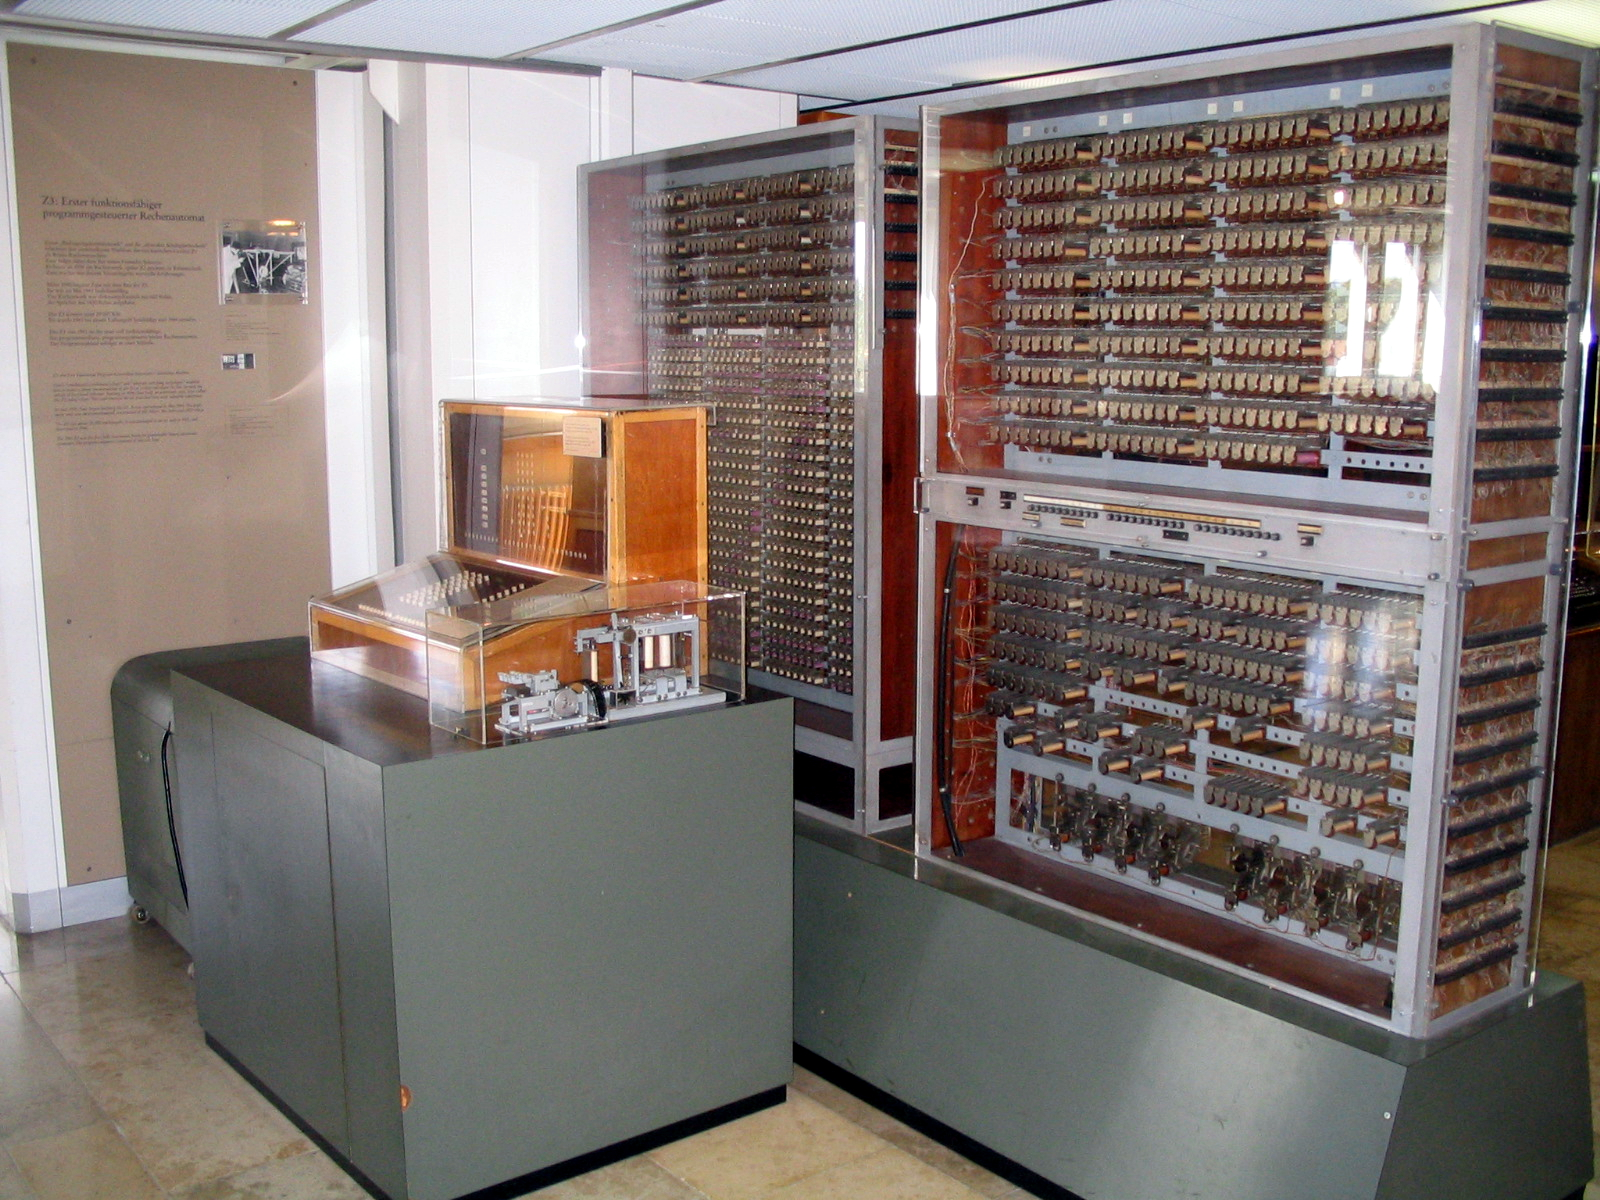
\includegraphics[width=22.22in]{images/Z3_Deutsches_Museum} \caption[Réplica de la Z3, la primer computadora con punto flotante (1941)]{Réplica de la Z3, la primer computadora con punto flotante (1941).}\label{fig:unnamed-chunk-61}
\end{marginfigure}

\begin{Shaded}
\begin{Highlighting}[]
\CommentTok{\#Veamos qué pasa con la suma}
\FunctionTok{options}\NormalTok{(}\AttributeTok{digits =} \DecValTok{22}\NormalTok{) }\CommentTok{\#Cambiamos dígitos}
\NormalTok{(}\FloatTok{0.1} \SpecialCharTok{+} \FloatTok{0.1} \SpecialCharTok{+} \FloatTok{0.1}\NormalTok{)    }\CommentTok{\#Sumamos}
\end{Highlighting}
\end{Shaded}

\begin{verbatim}
## [1] 0.3000000000000000444089
\end{verbatim}

\begin{marginfigure}
El comando \texttt{options(digits\ =\ 22)} especifica que \texttt{R}
debe imprimir en la consola \texttt{22} dígitos. No más. Si quieres
devolverlo a como lo tenías haz \texttt{options(digits\ =\ 7)}.
\end{marginfigure}

¡\href{https://www.youtube.com/watch?v=1jaCpeXg-gg}{Ahí está el
detalle}! \texttt{R} no sabe sumar. En general, ningún programa de
computadora sabe hacerlo. Veamos otros ejemplos:

\begin{Shaded}
\begin{Highlighting}[]
\FloatTok{4.1} \SpecialCharTok{{-}} \FloatTok{0.1} \CommentTok{\#Debería dar 4}
\end{Highlighting}
\end{Shaded}

\begin{verbatim}
## [1] 3.999999999999999555911
\end{verbatim}

\begin{Shaded}
\begin{Highlighting}[]
\DecValTok{3}\SpecialCharTok{/}\DecValTok{10}      \CommentTok{\#Debería ser 0.3}
\end{Highlighting}
\end{Shaded}

\begin{verbatim}
## [1] 0.2999999999999999888978
\end{verbatim}

\begin{Shaded}
\begin{Highlighting}[]
\FunctionTok{log}\NormalTok{(}\DecValTok{10}\SpecialCharTok{\^{}}\NormalTok{(}\DecValTok{12345}\NormalTok{), }\AttributeTok{base =} \DecValTok{10}\NormalTok{) }\CommentTok{\#Debería dar 12345}
\end{Highlighting}
\end{Shaded}

\begin{verbatim}
## [1] Inf
\end{verbatim}

El problema está en cómo las computadoras representan los números. Ellas
escriben los números en binario. Por ejemplo, 230 lo representan como
11100110 mientras que el 7 es: 111. El problema de las computadoras
radica en que éstas tienen una memoria finita por lo que números muy
grandes como: \(124765731467098372654176\) la computadora hace lo mejor
por representarlos eligiendo el más cercano:

\begin{Shaded}
\begin{Highlighting}[]
\CommentTok{\#Nota la diferencia entre lo que le decimos a R}
\CommentTok{\#y lo que resulta}
\NormalTok{x }\OtherTok{\textless{}{-}} \DecValTok{124765731467098372654176}
\NormalTok{x}
\end{Highlighting}
\end{Shaded}

\begin{verbatim}
## [1] 124765731467098377420800
\end{verbatim}

\begin{marginfigure}
Un error de punto flotante en la vida real ocasionó en los años noventa,
\href{https://www.esa.int/Newsroom/Press_Releases/Ariane_501_-_Presentation_of_Inquiry_Board_report}{la
explosión del cohete \texttt{Ariane\ 5}}. Moraleja: hay que tener
cuidado y respeto al punto flotante.
\end{marginfigure}

No olvides cambiar la cantidad de dígitos que deseas que imprima
\texttt{R} en su consola de vuelta:

\begin{Shaded}
\begin{Highlighting}[]
\FunctionTok{options}\NormalTok{(}\AttributeTok{digits =} \DecValTok{7}\NormalTok{) }\CommentTok{\#Cambiamos dígitos}
\end{Highlighting}
\end{Shaded}

El mismo problema ocurre con números decimales cuya representación
binaria es periódica; por ejemplo el \(\frac{1}{10}\) en binario se
representa como \(0.0001100110011\overline{0011}\dots\). Como es el
cuento de nunca acabar con dicho número, \texttt{R} lo trunca y almacena
sólo los primeros dígitos de ahí que, cada vez que escribes
\texttt{0.1}, \texttt{R} en realidad almacene el
0.1000000000000000055511 que es \emph{casi lo mismo} pero no es
estrictamente igual. Hay que tener mucho cuidado con esta inexactitud de
las computadoras (inexactitud estudiada por la rama de
\href{https://www.springer.com/gp/book/9781461484523}{Análisis
Numérico}) pues puede generar varios resultados imprevistos.

\hypertarget{cuxf3mo-checar-un-if}{%
\subsection{¿Cómo checar un if?}\label{cuxf3mo-checar-un-if}}

En general lo que hacen las computadoras para comparar valores es que
verifican que, en valor absoluto, el error sea pequeño. Recuerda que el
valor absoluto de \(x\), \(|x|\), regresa siempre el positivo: \[
|4| = 4 \qquad \textrm{y} \qquad |-8| = 8
\]

Para verificar que algo es más o menos \(0.3\) suele usarse el valor
absoluto\footnote{En \texttt{R} el comando \texttt{abs} toma el valor
  absoluto.} de la siguiente manera:

\begin{Shaded}
\begin{Highlighting}[]
\FunctionTok{abs}\NormalTok{( (}\FloatTok{0.1} \SpecialCharTok{+} \FloatTok{0.1} \SpecialCharTok{+} \FloatTok{0.1}\NormalTok{) }\SpecialCharTok{{-}} \FloatTok{0.3}\NormalTok{ ) }\SpecialCharTok{\textless{}} \DecValTok{1}\NormalTok{.e}\DecValTok{{-}6}
\end{Highlighting}
\end{Shaded}

\begin{verbatim}
## [1] TRUE
\end{verbatim}

donde \texttt{1.e-6} es notación corta para 0.000001 (también escrito
como \(1\times 10^{-6}\)). La pregunta que nos estamos haciendo es que
si el error entre sumar \(0.1+0.1+0.1\) y \(0.3\) es muy pequeño
\(< 0.000001\): \[
| (0.1 + 0.1 + 0.1) - 0.3 | < 0.000001
\]

\hypertarget{leer-y-almacenar-variables-en-r}{%
\chapter{\texorpdfstring{Leer y almacenar variables en
\texttt{R}}{Leer y almacenar variables en R}}\label{leer-y-almacenar-variables-en-r}}

Para terminar esta sección, aprenderemos cómo guardar variables en
\texttt{R}. Para eso, el concepto de directorio es uno de los más
relevantes. En general, en computación,
\href{https://en.wikipedia.org/wiki/Working_directory}{el directorio} se
refiere a la dirección en tu computadora donde estás trabajando. Por
ejemplo, si estás en una carpeta en tu escritorio de nombre
``Ejercicios\_R'' probablemente tu directorio sea
`\textasciitilde/Desktop/Ejercicios\_R/' (en Mac) o bien
`\textasciitilde\textbackslash Desktop\textbackslash Ejercicios\_R\textbackslash{}'
en Windows\footnote{Windows usa backslash. Y hay
  \href{https://www.howtogeek.com/181774/why-windows-uses-backslashes-and-everything-else-uses-forward-slashes/}{toda
  una historia detrás de ello}}. La forma de saber tu directorio (en
general) es ir a la carpeta que te interesa y con clic derecho ver
propiedades (o escribir \texttt{ls} en la terminal \texttt{Unix}).

\texttt{R} tiene un directorio \texttt{default} que quién sabe dónde
está (depende de tu instalación, generalmente está donde tu
\texttt{Usuario}). Usualmente lo mejor es elegir un directorio para cada
uno de los proyectos que hagas. Para ello si estás en \texttt{RStudio}
puedes utilizar \texttt{Shift+Ctrl+H} (\texttt{Shift+Cmd+H} en Mac) o
bien ir a
\texttt{Session\ \textgreater{}\ Set\ Working\ Directory\ \textgreater{}\ Choose\ Directory}
y elegir el directorio donde deseas trabajar tu proyecto. Pensando que
elegiste el escritorio (\texttt{Desktop} en mi computadora) notarás que
en la consola aparece el comando
\texttt{setwd("\textasciitilde{}/Desktop")} (o bien con
`\textbackslash{}' si eres Windows). Mi sugerencia es que copies ese
comando en tu \texttt{Script} para que, la próxima vez que lo corras ya
tengas preestablecido el directorio.

\begin{Shaded}
\begin{Highlighting}[]
\CommentTok{\#Si eres Mac/Linux}
\FunctionTok{setwd}\NormalTok{(}\StringTok{"\textasciitilde{}/Desktop"}\NormalTok{) }

\CommentTok{\#Si eres Windows}
\FunctionTok{setwd}\NormalTok{(}\StringTok{"C:\textbackslash{}Users\textbackslash{}Rodrigo\textbackslash{}Desktop"}\NormalTok{) }\CommentTok{\#Rodrigo = Mi usuario}
\end{Highlighting}
\end{Shaded}

\begin{verbatim}
## Error in setwd(escritorio): object 'escritorio' not found
\end{verbatim}

Podemos verificar el directorio elegido con \texttt{getwd()}:

\begin{Shaded}
\begin{Highlighting}[]
\FunctionTok{getwd}\NormalTok{()}
\end{Highlighting}
\end{Shaded}

\begin{marginfigure}
En general es buena práctica en \texttt{R} establecer, hasta arriba del
\texttt{Script}, el comando de directorio. Esto con el propósito de que,
cuando compartas un archivo, la persona a quien le fue compartido el
archivo pueda rápidamente elegir su propio directorio en su computadora.
\end{marginfigure}

Probemos guardar unas variables en un archivo dentro de nuestro
directorio. Para ello utilizaremos el comando \texttt{save}.

\begin{Shaded}
\begin{Highlighting}[]
\CommentTok{\#Crear las variables}
\NormalTok{x }\OtherTok{\textless{}{-}} \DecValTok{200}
\NormalTok{y }\OtherTok{\textless{}{-}} \DecValTok{100}

\CommentTok{\#Los archivos de variables de R son rda}
\FunctionTok{save}\NormalTok{(x,y, }\AttributeTok{file =} \StringTok{"MisVariables.rda"}\NormalTok{)}
\end{Highlighting}
\end{Shaded}

Si vas a tu directorio, notarás que el archivo \texttt{MisVariables.rda}
acaba de ser creado. De esta forma \texttt{R} puede almacenar objetos
creados en \texttt{R} que sólo \texttt{R} puede leer (más adelante
veremos cómo exportar bases de datos y gráficas). Observa que en tu
ambiente (si estás en \texttt{RStudio} puedes verlas en el panel 3)
deben aparecer las variables que hemos usado hasta ahora:

\begin{verbatim}
## [1] "x"        "y"        "z"        "Example1"
\end{verbatim}

Podemos probar sumar nuestras variables y todo funciona súper:

\begin{Shaded}
\begin{Highlighting}[]
\NormalTok{x }\SpecialCharTok{+}\NormalTok{ y }\CommentTok{\#Funciona magnífico}
\end{Highlighting}
\end{Shaded}

\begin{verbatim}
## [1] 300
\end{verbatim}

Limpiemos el ambiente. El comando equivalente al \texttt{clear\ all} en
\texttt{R} es un poco más complicado de memorizar:

\begin{Shaded}
\begin{Highlighting}[]
\CommentTok{\#EL clear all de R}
\FunctionTok{rm}\NormalTok{(}\AttributeTok{list =} \FunctionTok{ls}\NormalTok{())}
\end{Highlighting}
\end{Shaded}

Ahora, si vuelves a ver el ambiente, éste estará vacío: ¡hemos limpiado
el historial! Nota que si intentamos operar con las variables,
\texttt{R} ya no las recuerda:

\begin{Shaded}
\begin{Highlighting}[]
\NormalTok{x }\SpecialCharTok{+}\NormalTok{ y }\CommentTok{\#Error}
\end{Highlighting}
\end{Shaded}

\begin{verbatim}
## Error in eval(expr, envir, enclos): object 'x' not found
\end{verbatim}

\begin{marginfigure}
Así como hay que lavarse las manos antes de comer, es buen hábito
limpiar todas las variables del ambiente de \texttt{R} antes de usarlo.
\end{marginfigure}

\begin{verbatim}
## 1 directory created.
\end{verbatim}

\begin{verbatim}
## 1 file moved. 0 failed.
\end{verbatim}

Podemos leer la base de datos usando \texttt{load}:

\begin{Shaded}
\begin{Highlighting}[]
\CommentTok{\#Leemos las variables}
\FunctionTok{load}\NormalTok{(}\StringTok{"MisVariables.rda"}\NormalTok{)}
\end{Highlighting}
\end{Shaded}

\begin{verbatim}
## Warning in readChar(con, 5L, useBytes = TRUE): cannot open compressed file
## 'MisVariables.rda', probable reason 'No such file or directory'
\end{verbatim}

\begin{verbatim}
## Error in readChar(con, 5L, useBytes = TRUE): cannot open the connection
\end{verbatim}

\begin{Shaded}
\begin{Highlighting}[]
\CommentTok{\#Una vez leídas podemos empezar a jugar con ellas}
\NormalTok{x }\SpecialCharTok{+}\NormalTok{ y }\CommentTok{\#Ya funciona}
\end{Highlighting}
\end{Shaded}

\begin{verbatim}
## Error in eval(expr, envir, enclos): object 'x' not found
\end{verbatim}

Por último, es necesario resaltar la importancia del directorio. Para
ello crea una nueva carpeta en tu escritorio de nombre
\texttt{"Mi\_curso\_de\_R"}. Mueve el archivo
\texttt{"MisVariables.rda"} dentro de la carpeta. Borra todo e intenta
leer de nuevo el archivo:

¡

\begin{Shaded}
\begin{Highlighting}[]
\CommentTok{\#Borramos todo}
\FunctionTok{rm}\NormalTok{(}\AttributeTok{list =} \FunctionTok{ls}\NormalTok{())}

\CommentTok{\#Intentamos leer el archivo de nuevo}
\FunctionTok{load}\NormalTok{(}\StringTok{"MisVariables.rda"}\NormalTok{)}
\end{Highlighting}
\end{Shaded}

\begin{verbatim}
## Warning in readChar(con, 5L, useBytes = TRUE): cannot open compressed file
## 'MisVariables.rda', probable reason 'No such file or directory'
\end{verbatim}

\begin{verbatim}
## Error in readChar(con, 5L, useBytes = TRUE): cannot open the connection
\end{verbatim}

Este error es porque \texttt{R} sigue pensando que nuestro directorio es
el escritorio y está buscando el archivo ahí sin hallarlo. Para
encontrarlo hay que cambiar el directorio a través de \texttt{RStudio}
(ya sea \texttt{Ctrl+Shift+H} o
\texttt{Session\ \textgreater{}Set\ Working\ Directory\ \textgreater{}\ Choose\ Directory})
o bien a través de comandos en \texttt{R}:

\begin{Shaded}
\begin{Highlighting}[]
\CommentTok{\#Si eres Mac/Linux}
\FunctionTok{setwd}\NormalTok{(}\StringTok{"\textasciitilde{}/Desktop/Mi\_curso\_de\_R"}\NormalTok{) }

\CommentTok{\#Si eres Windows}
\FunctionTok{setwd}\NormalTok{(}\StringTok{"C:\textbackslash{}Users\textbackslash{}Rodrigo\textbackslash{}Desktop\textbackslash{}Mi\_curso\_de\_R"}\NormalTok{) }\CommentTok{\#Rodrigo = Mi usuario}
\end{Highlighting}
\end{Shaded}

\begin{Shaded}
\begin{Highlighting}[]
\FunctionTok{file.move}\NormalTok{( }\FunctionTok{paste0}\NormalTok{(subdir,}\StringTok{"/"}\NormalTok{, }\StringTok{"MisVariables.rda"}\NormalTok{), }\StringTok{"MisVariables.rda"}\NormalTok{)}
\end{Highlighting}
\end{Shaded}

\begin{verbatim}
## Error in paste0(subdir, "/", "MisVariables.rda"): object 'subdir' not found
\end{verbatim}

\begin{Shaded}
\begin{Highlighting}[]
\CommentTok{\#Aquí sí se puede leer}
\FunctionTok{load}\NormalTok{(}\StringTok{"MisVariables.rda"}\NormalTok{)}
\end{Highlighting}
\end{Shaded}

\begin{verbatim}
## Warning in readChar(con, 5L, useBytes = TRUE): cannot open compressed file
## 'MisVariables.rda', probable reason 'No such file or directory'
\end{verbatim}

\begin{verbatim}
## Error in readChar(con, 5L, useBytes = TRUE): cannot open the connection
\end{verbatim}

\hypertarget{ejercicio-2}{%
\subsection{Ejercicio}\label{ejercicio-2}}

Responde a las siguientes preguntas:

\begin{enumerate}
\def\labelenumi{\arabic{enumi}.}
\item
  ¿Qué es el directorio y por qué es necesario establecerlo?
\item
  Si \texttt{R} me da el error
  \texttt{\textquotesingle{}No\ such\ file\ or\ directory\textquotesingle{}}
  ¿qué hice mal?
\item
  En \texttt{RStudio}, ¿qué hace
  \texttt{Session\ \textgreater{}\ Restart\ R}? ¿cuál es la diferencia
  con \texttt{rm(list\ =\ ls())}?
\item
  ¿Qué hace el comando \texttt{cat("\textbackslash{}014")}? (\emph{Ojo}
  puede que no haga nada). Si funciona, ¿cuál es la diferencia con
  \texttt{rm(list\ =\ ls())} y con \texttt{Restart\ R}?
\end{enumerate}

\hypertarget{instalaciuxf3n-de-paquetes}{%
\chapter{Instalación de paquetes}\label{instalaciuxf3n-de-paquetes}}

Un paquete de \texttt{R} es un conjunto de funciones adicionales
elaboradas por los usuarios, las cuales permiten hacer cosas adicionales
en \texttt{R}. Para instalarlos requieres de una conexión a Internet (o
bien puedes instalarlos a partir de un archivo, por ejemplo, mediante
una \texttt{USB}). El comando de instalación es
\texttt{install.packages} seguido del nombre del paquete. Por ejemplo (y
por ocio) descarguemos el paquete \texttt{beepr} para hacer reproducir
sonidos en la computadora\footnote{En los siguientes capítulos
  descargaremos paquetes más interesantes; pero no desprecies la
  utilidad de \texttt{beepr} yo lo he usado en múltiples ocasiones para
  que la computadora me avise que ya terminó de correr un código.}. Para
ello:

\begin{Shaded}
\begin{Highlighting}[]
\FunctionTok{install.packages}\NormalTok{(}\StringTok{"beepr"}\NormalTok{)}
\end{Highlighting}
\end{Shaded}

\begin{verbatim}
[...]
* DONE (beepr)

The downloaded source packages are in
    ‘/algun/lugar/downloaded_packages’
\end{verbatim}

Esto significa que el paquete ha sido instalado. Nos interesa usar la
función \texttt{beep} que emite un sonido (\texttt{??beep} para ver la
ayuda). Si la llamamos así tal cual, nos da error:

\begin{Shaded}
\begin{Highlighting}[]
\FunctionTok{beep}\NormalTok{(}\DecValTok{3}\NormalTok{)}
\end{Highlighting}
\end{Shaded}

\texttt{R} es incapaz de hallar la función porque aún no le hemos dicho
dónde se encuentra. Para ello podemos llamar al paquete mediante la
función \texttt{library} y decirle a \texttt{R} que incluya las
funciones que se encuentran dentro de \texttt{beepr}:

\begin{Shaded}
\begin{Highlighting}[]
\FunctionTok{library}\NormalTok{(beepr)}
\FunctionTok{beep}\NormalTok{(}\DecValTok{3}\NormalTok{) }\CommentTok{\#Esto produce un sonido}
\end{Highlighting}
\end{Shaded}

El comando \texttt{library} le dice a \texttt{R} ¡hey, voy a usar unas
funciones que creó alguien más y que están dentro del paquete
\texttt{beepr}! De esta manera, al correr \texttt{beep(3)}, \texttt{R}
ya sabe dónde hallar la función y por eso no arroja error.

\hypertarget{ejercicios-1}{%
\subsection{Ejercicios}\label{ejercicios-1}}

\textbf{NIVEL 1}

\begin{enumerate}
\def\labelenumi{\arabic{enumi}.}
\tightlist
\item
  Instala los paquetes \texttt{tidyverse} en \texttt{R}.
\item
  De \texttt{tidyverse} haz lo necesario para que el siguiente bloque de
  código te arroje una gráfica:
\end{enumerate}

\begin{Shaded}
\begin{Highlighting}[]
\CommentTok{\#Aquí tienes que hacer algo}
\CommentTok{\#}
\CommentTok{\# RELLENA AQUÍ}
\CommentTok{\#}

\CommentTok{\#Esto genera un histograma}
\FunctionTok{set.seed}\NormalTok{(}\DecValTok{1364752}\NormalTok{)}
\NormalTok{mis.datos }\OtherTok{\textless{}{-}} \FunctionTok{data.frame}\NormalTok{(}\AttributeTok{x =} \FunctionTok{rnorm}\NormalTok{(}\DecValTok{1000}\NormalTok{))}
\FunctionTok{ggplot}\NormalTok{(mis.datos, }\FunctionTok{aes}\NormalTok{(}\AttributeTok{x =}\NormalTok{ x)) }\SpecialCharTok{+} 
  \FunctionTok{geom\_histogram}\NormalTok{(}\AttributeTok{bins =} \DecValTok{50}\NormalTok{, }\AttributeTok{fill =} \StringTok{"deepskyblue3"}\NormalTok{) }\SpecialCharTok{+}
  \FunctionTok{ggtitle}\NormalTok{(}\StringTok{"Histograma generado por el código"}\NormalTok{)}
\end{Highlighting}
\end{Shaded}

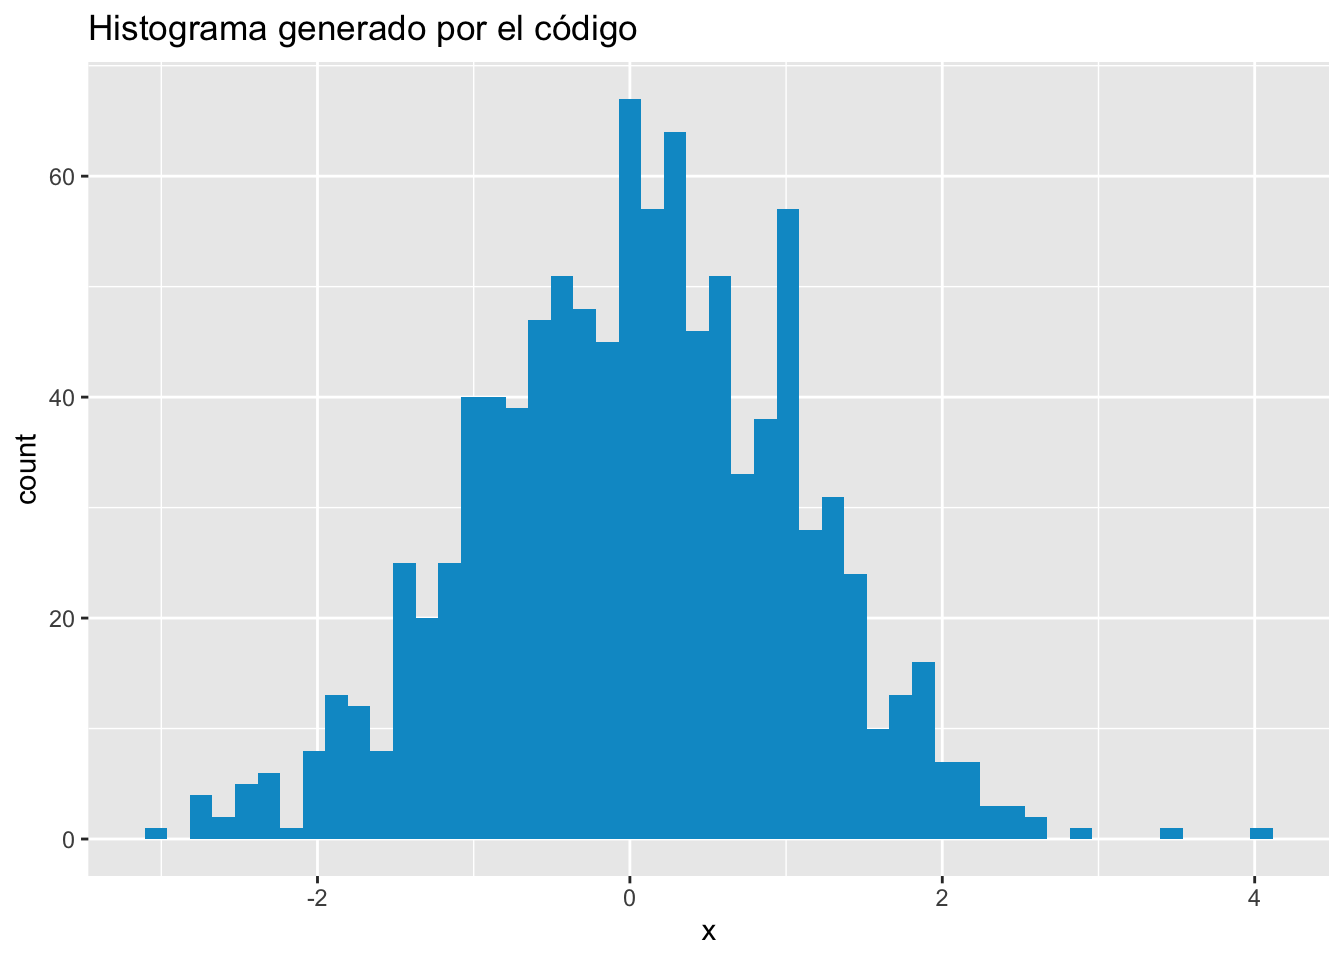
\includegraphics{Introducción_a_R_files/figure-latex/unnamed-chunk-89-1}

\textbf{NIVEL 3}

\begin{enumerate}
\def\labelenumi{\arabic{enumi}.}
\tightlist
\item
  Instala el paquete \texttt{devtools} (para hacerlo probablemente
  necesites instalar más cosas en tu computadora; averigua cuáles)
\item
  Usa \texttt{devtools} para instalar el paquete
  \href{https://github.com/dill/emoGG}{\texttt{emoGG}} desde Github.
\item
  Verifica que tu instalación fue correcta haciendo la siguiente
  gráfica:
\end{enumerate}

\begin{Shaded}
\begin{Highlighting}[]
\FunctionTok{library}\NormalTok{(emoGG)}
\FunctionTok{ggplot}\NormalTok{(mtcars, }\FunctionTok{aes}\NormalTok{(wt, mpg))}\SpecialCharTok{+} \FunctionTok{geom\_emoji}\NormalTok{(}\AttributeTok{emoji=}\StringTok{"1f697"}\NormalTok{)}
\end{Highlighting}
\end{Shaded}

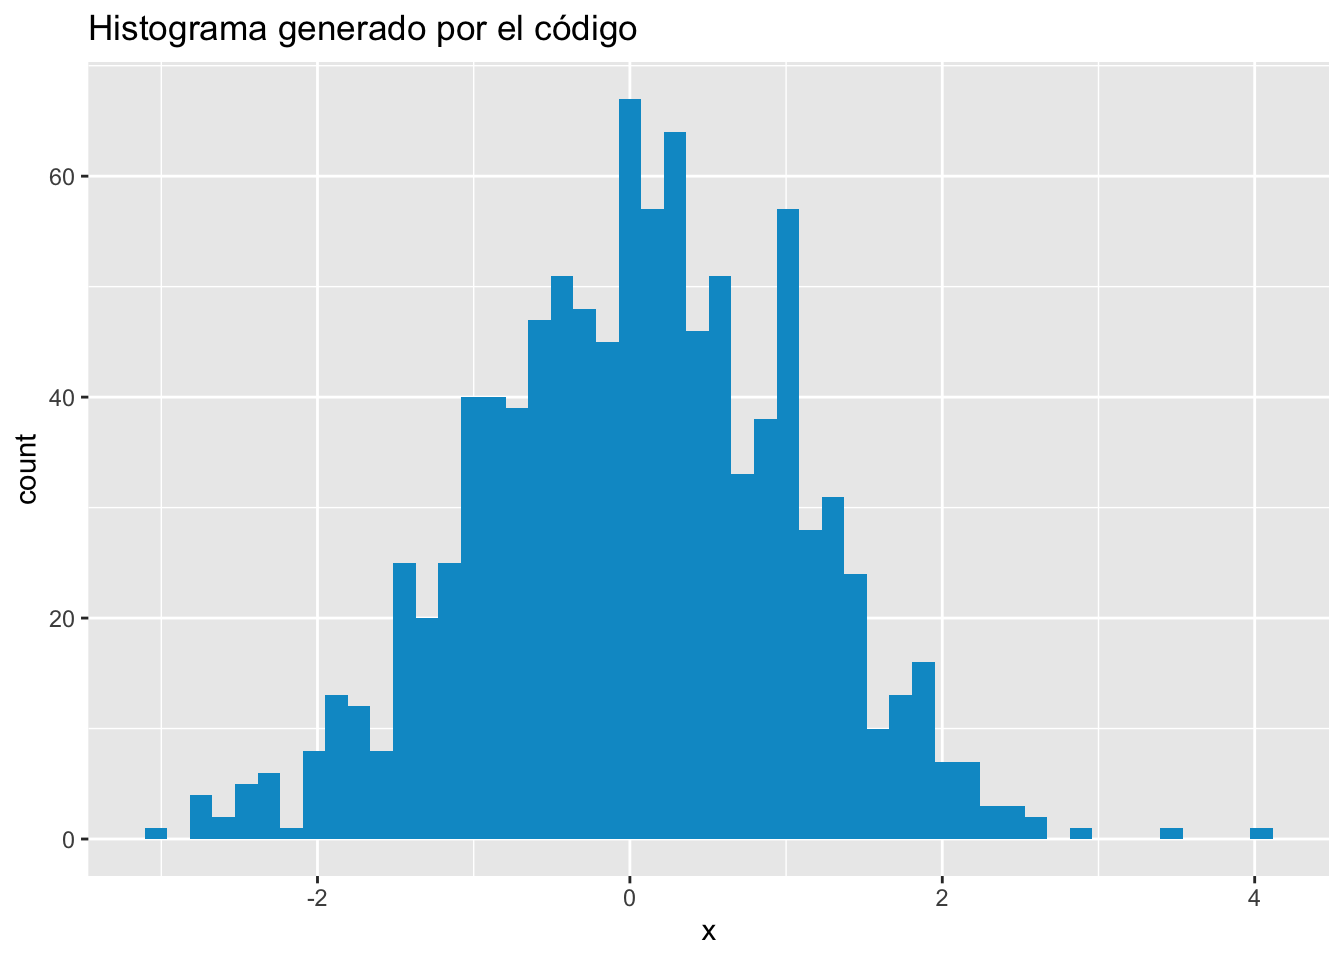
\includegraphics{Introducción_a_R_files/figure-latex/unnamed-chunk-90-1}

\hypertarget{comentarios-adicionales-sobre-el-formato}{%
\chapter{Comentarios adicionales sobre el
formato}\label{comentarios-adicionales-sobre-el-formato}}

Así como en el español existen reglas de gramática para ponernos todos
de acuerdo y entendernos entre todos, en \texttt{R} también existen
\emph{sugerencias} a seguir para escribir tu código. Las sugerencias que
aquí aparecen fueron adaptadas de las que
\href{https://google.github.io/styleguide/Rguide.xml}{utiliza el equipo
de \texttt{Google}}.

\begin{enumerate}
\def\labelenumi{\arabic{enumi}.}
\item
  No escribas líneas de más de 80 caracteres (si se salió de tu
  pantalla, mejor continúa en el siguiente renglón).
\item
  Coloca espacios entre operadores
  \texttt{+,*,/,-,\textless{}-,=,\ \textless{},\ \textless{}=,\ \textgreater{},\ \textgreater{}=,\ ==}
  y usa paréntesis para agrupar:
\end{enumerate}

\begin{Shaded}
\begin{Highlighting}[]
\CommentTok{\#Esto no se ve muy bien}
\FunctionTok{abs}\NormalTok{(}\DecValTok{3}\SpecialCharTok{*}\DecValTok{5}\SpecialCharTok{/}\NormalTok{(}\DecValTok{4{-}9}\NormalTok{)}\SpecialCharTok{\^{}}\DecValTok{2{-}60}\SpecialCharTok{/}\DecValTok{100{-}888}\FloatTok{+0.1}\SpecialCharTok{*}\DecValTok{8888{-}4}\SpecialCharTok{/}\DecValTok{10}\SpecialCharTok{*}\DecValTok{2}\NormalTok{) }\SpecialCharTok{\textless{}} \DecValTok{1}\NormalTok{.e}\DecValTok{{-}6}

\CommentTok{\#Los espacios permiten distinguir el orden de las operaciones}
\FunctionTok{abs}\NormalTok{( (}\DecValTok{3} \SpecialCharTok{*} \DecValTok{5}\NormalTok{) }\SpecialCharTok{/}\NormalTok{ (}\DecValTok{4} \SpecialCharTok{{-}} \DecValTok{9}\NormalTok{)}\SpecialCharTok{\^{}}\DecValTok{2} \SpecialCharTok{{-}} \DecValTok{60} \SpecialCharTok{/} \DecValTok{100} \SpecialCharTok{{-}} \DecValTok{888} 
      \SpecialCharTok{+}\NormalTok{ (}\FloatTok{0.1} \SpecialCharTok{*} \DecValTok{8888}\NormalTok{) }\SpecialCharTok{{-}}\NormalTok{ (}\DecValTok{4} \SpecialCharTok{/} \DecValTok{10}\NormalTok{) }\SpecialCharTok{*} \DecValTok{2}\NormalTok{ ) }\SpecialCharTok{\textless{}} \DecValTok{1}\NormalTok{.e}\DecValTok{{-}6}
\end{Highlighting}
\end{Shaded}

\begin{enumerate}
\def\labelenumi{\arabic{enumi}.}
\setcounter{enumi}{2}
\tightlist
\item
  Intenta alinear la asignación de variables para legibilidad:
\end{enumerate}

\begin{Shaded}
\begin{Highlighting}[]
\CommentTok{\#Esto no tanto}
\NormalTok{altura }\OtherTok{\textless{}{-}} \FloatTok{1.80}
\NormalTok{peso }\OtherTok{\textless{}{-}} \DecValTok{80}
\NormalTok{edad }\OtherTok{\textless{}{-}} \DecValTok{32}

\CommentTok{\#Esto se ve bien}
\NormalTok{altura }\OtherTok{\textless{}{-}} \FloatTok{1.80}
\NormalTok{peso   }\OtherTok{\textless{}{-}} \DecValTok{80}
\NormalTok{edad   }\OtherTok{\textless{}{-}} \DecValTok{32}
\end{Highlighting}
\end{Shaded}

\begin{enumerate}
\def\labelenumi{\arabic{enumi}.}
\setcounter{enumi}{3}
\tightlist
\item
  Utiliza nombres que evoquen la variable que representas
\end{enumerate}

\begin{Shaded}
\begin{Highlighting}[]
\CommentTok{\#Cuando regreses a esto no sabrás ni qué}
\NormalTok{x }\OtherTok{\textless{}{-}} \DecValTok{10}
\NormalTok{y }\OtherTok{\textless{}{-}} \DecValTok{2}
\NormalTok{z }\OtherTok{\textless{}{-}} \FloatTok{3.14}
\NormalTok{W }\OtherTok{\textless{}{-}}\NormalTok{ z }\SpecialCharTok{*}\NormalTok{ x}\SpecialCharTok{\^{}}\NormalTok{y }\CommentTok{\#¿Qué calculé?}

\CommentTok{\#Es mejor especificar la variable}
\NormalTok{radio        }\OtherTok{\textless{}{-}} \DecValTok{10}
\NormalTok{potencia     }\OtherTok{\textless{}{-}} \DecValTok{2}
\NormalTok{pi\_aprox     }\OtherTok{\textless{}{-}} \FloatTok{3.14}
\NormalTok{area\_circulo }\OtherTok{\textless{}{-}}\NormalTok{ pi\_aprox }\SpecialCharTok{*}\NormalTok{ radio}\SpecialCharTok{\^{}}\NormalTok{potencia}
\end{Highlighting}
\end{Shaded}

\begin{enumerate}
\def\labelenumi{\arabic{enumi}.}
\setcounter{enumi}{4}
\tightlist
\item
  No utilices un nombre demasiado similar para cosas diferentes.
\end{enumerate}

\begin{Shaded}
\begin{Highlighting}[]
\CommentTok{\#Aquí, seguro eventualmente te vas a equivocar}
\NormalTok{altura }\OtherTok{\textless{}{-}} \DecValTok{10}   \CommentTok{\#Altura del edificio}
\NormalTok{Altura }\OtherTok{\textless{}{-}} \FloatTok{1.8}  \CommentTok{\#Mi altura}
\NormalTok{ALTURA }\OtherTok{\textless{}{-}} \DecValTok{2000} \CommentTok{\#La altitud de la CDMX}

\CommentTok{\#Siempre elegir nombres claros, aunque largos}
\NormalTok{altura.edificio }\OtherTok{\textless{}{-}} \DecValTok{10}   \CommentTok{\#Altura del edificio}
\NormalTok{altura.Rodrigo  }\OtherTok{\textless{}{-}} \FloatTok{1.8}  \CommentTok{\#Mi altura}
\NormalTok{altura.CDMX     }\OtherTok{\textless{}{-}} \DecValTok{2000} \CommentTok{\#La altitud de la CDMX}
\end{Highlighting}
\end{Shaded}

\begin{enumerate}
\def\labelenumi{\arabic{enumi}.}
\setcounter{enumi}{5}
\tightlist
\item
  Comenta:
\end{enumerate}

\begin{Shaded}
\begin{Highlighting}[]
\CommentTok{\#¿Qué hace esto?}
\NormalTok{x }\OtherTok{\textless{}{-}} \DecValTok{168}
\NormalTok{x }\OtherTok{\textless{}{-}}\NormalTok{ x}\SpecialCharTok{/}\DecValTok{100}
\NormalTok{y }\OtherTok{\textless{}{-}} \FloatTok{71.2}
\FunctionTok{print}\NormalTok{(y}\SpecialCharTok{/}\NormalTok{x}\SpecialCharTok{\^{}}\DecValTok{2}\NormalTok{) }
  
\CommentTok{\#Es mejor así}
\NormalTok{altura }\OtherTok{\textless{}{-}} \DecValTok{168}        \CommentTok{\#en centímetros}
\NormalTok{altura }\OtherTok{\textless{}{-}}\NormalTok{ altura}\SpecialCharTok{/}\DecValTok{100} \CommentTok{\#en metros}
\NormalTok{peso   }\OtherTok{\textless{}{-}} \FloatTok{71.2}       \CommentTok{\#peso en kg}
\FunctionTok{print}\NormalTok{(peso}\SpecialCharTok{/}\NormalTok{altura}\SpecialCharTok{\^{}}\DecValTok{2}\NormalTok{) }\CommentTok{\#índice masa corporal}
\end{Highlighting}
\end{Shaded}

\begin{marginfigure}

\includegraphics[width=10in]{images/tweet1} \caption[Trad]{Trad: Un periodista se acerca a un programador a preguntarle ¿qué hace que un código sea malo? -Sin comentarios.}\label{fig:unnamed-chunk-96}
\end{marginfigure}

\begin{enumerate}
\def\labelenumi{\arabic{enumi}.}
\setcounter{enumi}{6}
\tightlist
\item
  Siempre pon las llamadas a los paquetes y el directorio al inicio de
  tu archivo para que otro usuario sepa qué necesita.
\end{enumerate}

Código limpio y legible:

\begin{Shaded}
\begin{Highlighting}[]
\CommentTok{\#Asumiendo aquí inicia el archivo:}
\FunctionTok{setwd}\NormalTok{(}\StringTok{"Mi directorio"}\NormalTok{)}

\CommentTok{\#Llamamos la librería}
\FunctionTok{library}\NormalTok{(beepr)}
\FunctionTok{library}\NormalTok{(tidyverse)}

\CommentTok{\#Analizamos una base de datos de R}
\FunctionTok{data}\NormalTok{(iris) }\CommentTok{\#Base de datos de flores}

\CommentTok{\#Agrupamos la base por especie}
\NormalTok{iris.agrupada }\OtherTok{\textless{}{-}} \FunctionTok{group\_by}\NormalTok{(iris, Species)}

\CommentTok{\#Obtenemos la media por longitud de sépalo}
\NormalTok{iris.media    }\OtherTok{\textless{}{-}} \FunctionTok{summarise}\NormalTok{(iris.agrupada, }\AttributeTok{SL.mean =} \FunctionTok{mean}\NormalTok{(Sepal.Length))}

\CommentTok{\#Avisa que ya terminó}
\FunctionTok{beep}\NormalTok{(}\DecValTok{5}\NormalTok{)}
\end{Highlighting}
\end{Shaded}

es siempre preferible a código escrito \emph{con prisas} :

\begin{marginfigure}

\includegraphics[width=8.89in]{images/Grandma-Finds-The-Internet} \caption[Yo, leyendo mi código no comentado y con mala edición 6 meses después de haberlo hecho]{Yo, leyendo mi código no comentado y con mala edición 6 meses después de haberlo hecho.}\label{fig:unnamed-chunk-98}
\end{marginfigure}

\begin{Shaded}
\begin{Highlighting}[]
\FunctionTok{data}\NormalTok{(iris);}\FunctionTok{setwd}\NormalTok{(}\StringTok{"Mi directorio"}\NormalTok{)}
\FunctionTok{library}\NormalTok{(tidyverse);x}\OtherTok{\textless{}{-}}\FunctionTok{group\_by}\NormalTok{(iris,Species  )}
\CommentTok{\#Aquí hacemos esto}
\NormalTok{iris.means}\OtherTok{=}\FunctionTok{summarise}\NormalTok{( x,}\AttributeTok{SL.mean=}\FunctionTok{mean}\NormalTok{(Sepal.Length));}\FunctionTok{library}\NormalTok{(beepr);}\FunctionTok{beep}\NormalTok{(}\DecValTok{5}\NormalTok{)}\CommentTok{\#FIN}
\end{Highlighting}
\end{Shaded}

Siempre escribe tu código pensando que alguien más
(\href{https://www.redaccionmedica.com/virico/noticias/el-gato-de-schrodinger-y-por-que-no-abrir-la-puerta-cerrada-de-la-consulta-5188}{y
ese alguien más puedes ser tú}) va a leerlo. ¡No olvides comentar!

\hypertarget{continuaciuxf3n}{%
\section{Continuación}\label{continuaciuxf3n}}

¡Felicidades! Ya terminaste esta sección. Puedes ir a:

\begin{itemize}
\tightlist
\item
  \href{Graficación_con_gglot2.html}{Graficación con \texttt{ggplot2}}.
\item
  \href{Estadística_Descriptiva.html}{Bases de datos y análisis
  descriptivo en \texttt{R}}.
\end{itemize}

\bibliography{skeleton.bib}



\end{document}
